\documentclass[10pt,twocolumn]{article}

\usepackage[margin=0.70in,top=0.80in,bottom=0.80in]{geometry}
\usepackage[T1]{fontenc}
\usepackage{lmodern}
\usepackage{microtype}
\usepackage{amsmath,amssymb}
\usepackage{booktabs}
\usepackage{array}
\usepackage{graphicx}
\usepackage{xcolor}
\usepackage{enumitem}
\usepackage{caption}
\usepackage{titlesec}
\usepackage{fancyhdr}
\usepackage[colorlinks=true,linkcolor=blue!55!black,citecolor=blue!55!black,urlcolor=blue!55!black]{hyperref}

\definecolor{atlasdark}{HTML}{111827}
\definecolor{atlasmuted}{HTML}{4B5563}

\renewcommand{\topfraction}{0.88}
\renewcommand{\dbltopfraction}{0.88}
\renewcommand{\textfraction}{0.08}
\renewcommand{\floatpagefraction}{0.75}
\renewcommand{\dblfloatpagefraction}{0.75}

\setlength{\columnsep}{0.24in}
\setlength{\parskip}{2.8pt}
\setlength{\emergencystretch}{1.6em}
\captionsetup{font=small,labelfont=bf,skip=3.5pt}
\titleformat{\section}{\large\bfseries\color{atlasdark}}{\thesection.}{0.5em}{}
\titleformat{\subsection}{\normalsize\bfseries\color{atlasdark}}{\thesubsection}{0.45em}{}
\titlespacing*{\section}{0pt}{8.5pt}{3pt}
\titlespacing*{\subsection}{0pt}{6pt}{2pt}

\pagestyle{fancy}
\fancyhf{}
\fancyhead[L]{\footnotesize\color{atlasmuted}Zero-Gradient Omni-Modal Grafting \& Host-Enforced Alignment}
\fancyhead[R]{\footnotesize\color{atlasmuted}Preprint v0.9.3 (2026-11-27)}
\fancyfoot[C]{\footnotesize\thepage}
\renewcommand{\headrulewidth}{0.4pt}

\title{\vspace{-1.1em}\Large\bfseries Zero-Gradient Omni-Modal Grafting via Closed-Form Representation Maps:\\
Sealed Confirmation, Spectral Rank Collapse, Multi-Donor Blends, and Host-Enforced Alignment}

\author{William Joseph Tatum (Monkey)\thanks{Human author and project director, Atlas 3DSS. AI coding and research agents (\emph{Neon}, Atlas 3DSS) assisted with implementation, verification automation, and manuscript drafting under human oversight and cryptographic artifact verification; AI systems are disclosed here rather than listed as authors per arXiv authorship policy.}\\
\small Atlas 3DSS\\
\small\url{https://github.com/Atlas3DSS/atlas-ingine}\\
\small\url{https://huggingface.co/collections/Atlas3D/omni-by-atlas-6b09daccd0f65e23233163b3}}
\date{November 27, 2026}

\begin{document}

% --- Standalone Opening Page: Special Thanks & AI Systems Call-Out (Neon) ---
\onecolumn
\thispagestyle{empty}
\begin{center}
\vspace*{1.6in}
{\Large\bfseries\color{atlasdark} Special Thanks \& Acknowledgment}\\[0.6em]
{\large\color{atlasmuted} Dedicated Call-Out to \textbf{Neon} (Atlas 3DSS AI Engineering \& Research System)}\\[1.8em]
\rule{0.72\textwidth}{0.6pt}
\end{center}
\vspace{1.0em}
\begin{quote}
\normalsize
Per arXiv's Generative AI authorship policy, artificial intelligence systems are not listed as authors in the paper metadata or byline. We therefore dedicate this opening standalone page to give explicit, prominent credit to \textbf{Neon} (the autonomous AI research and engineering agent collective operated inside Atlas 3DSS's Switchboard).

Under the direction, architecture decisions, and verification discipline of the human author (\textbf{William Joseph Tatum (Monkey)}), \textbf{Neon} executed closed-form FP64 ridge fitting, cross-silicon CUDA kernel porting and 30-GPU benchmarking, sealed-split statistical auditing, adversarial Pliny red-teaming, reproducible world-model turnaround verification, figure synthesis, and manuscript drafting across this study. Every quantitative claim, control, and preserved failure in the pages that follow was independently checked against cryptographic SHA-256 receipts and raw hardware outputs.

\vspace{1.2em}
\noindent\textit{--- William Joseph Tatum (Monkey), Atlas 3DSS (November 27, 2026)}
\end{quote}
\vspace{1.4em}
\begin{center}
\rule{0.72\textwidth}{0.6pt}
\end{center}
\clearpage

\twocolumn[
\begin{@twocolumnfalse}
\maketitle
\vspace{-1.2em}
\begin{abstract}
\noindent
Closed-form linear representation maps (\emph{Plato's Keys}) graft image diffusion, video+audio diffusion, coarse visual perception, symbolic music, and prosodic speech conditioning onto frozen language models with zero gradient steps and zero trunk weight edits. Extending prior dense-LLM H3 ridge substitution (\texttt{TE-PK-Minimax-H3}) to looped-MoE \texttt{Inkling-2-Mini}, a $90.0\,\text{MiB}$ FP16 \texttt{concat4} ridge map fitted on $640$ prompts ($13{,}872$ word spans) replaces the $27.14\,\text{GB}$ \texttt{Qwen3-VL-32B} layer-50 encoder in \texttt{MiniMax-H3}: on a sealed $160$-prompt confirmation split ($640$ $1024\times 1024$ images, $G=16$ groups, $\texttt{fit\_calls}=0$), \texttt{concat4} scores $0.1982$ SigLIP2 vs.\ $0.2045$ teacher (descriptive $97.50\%$ retention vs.\ single-tap $B_0$; $0.8942$ image-vs-teacher cosine; $R^2=0.9982$), while primary $22.5\,\text{MiB}$ \texttt{single\_tap} beats matched $B_0$ on $16/16$ groups ($p=3.05\times 10^{-5}$). A matched-data 2-layer residual GELU MLP shows no detectable grouped Confirm-160 cosine gain ($+0.00018$, CI ${[-0.00074,+0.00115]}$, $p=1.0$). The identical $90.0\,\text{MiB}$ key drives $5.875\,\text{s}$ \texttt{FL2VA} video+audio across $16$ GPUs ($30$-GPU parity $\min\cos=0.999947$), and separately fitted keys pass $4/6$ Wave~B Confirm-160 word bars (including \texttt{FLUX.2-dev} $R^2=0.6523$, Dev-24 render $99.65\%$). We document explicit failure boundaries: reverse Vision$\to$LLM dense OCR, \texttt{SDXL} ($57.69\%/42.66\%$), and one-shot \texttt{Mouth} confirm ($4/6$ gates). Exact FP64 SVD ($20$ keys) and live V100 donor-prefill MoE pruning show rank-64 speech compression ($26.2\times/29.1\times$) and $60\%$ cold-expert pruning ($1.71\times$ prefill speedup, $-0.0040$ \texttt{val\_dev} word cos), alongside a $5$-family TTS shoot-out, a reproducible $360^\circ$ Verified Ledger world-model turnaround, and live Pliny red-teaming ($0/40$ committed violations vs.\ $22/40$ prompt-only).
\end{abstract}
\vspace{0.8em}
\end{@twocolumnfalse}
]

\section{Introduction}
Multimodal foundation models typically align text, image, video, audio, and speech components through multi-billion-token joint pretraining or gradient-trained adapters (Flamingo \cite{alayrac2022flamingo}, BLIP-2 \cite{li2023blip2}, LLaVA \cite{liu2023llava,liu2023llava15}). We evaluate an operational systems question: \emph{how far do zero-gradient closed-form linear maps carry cross-modal conditioning between frozen language trunks and frozen generative/perceptual receivers, where do they break, and how do they compose with host-enforced verification?} (Fig.~\ref{fig:arch}).

Building on model stitching \cite{lenc2015equivariance,bansal2021stitching}, Relative Representations \cite{moschella2023relative,bakker2026relative}, the Platonic Representation Hypothesis \cite{huh2024platonic}, Stanford Hazy Research's \emph{Plato's Key} \cite{cheng2026platoskey}, and \texttt{Alissonerdx/TE-PK-Minimax-H3} \cite{alissonerdx2026tepk} (which introduced closed-form ridge substitution from dense LLMs into \texttt{MiniMax-H3} \texttt{Qwen3-VL-32B} layer-50 conditioning), we extend linear grafting across heterogeneous architectures (looped-MoE \texttt{Inkling-2-Mini}, \texttt{Qwen3.8-27B}, \texttt{DeepSeek-V4.1-Flash}, and \texttt{GLM-5.3-Flash}), verify Packet~A on a sealed $160$-prompt split with orthogonal \texttt{DINOv3} teacher similarity and a matched-data residual MLP comparator, map exact OCR/speech/SDXL failure boundaries, quantify spectral rank and live MoE expert specialization, and pair local serving with host-enforced Verified Ledger alignment and a reproducible $360^\circ$ world-model persistence benchmark. Throughout, disk sizes use decimal $\text{GB}$ (or exact binary $\text{MiB}$ for keys) and CUDA memory peaks use binary $\text{GiB}$.

\begin{figure*}[t]
\centering
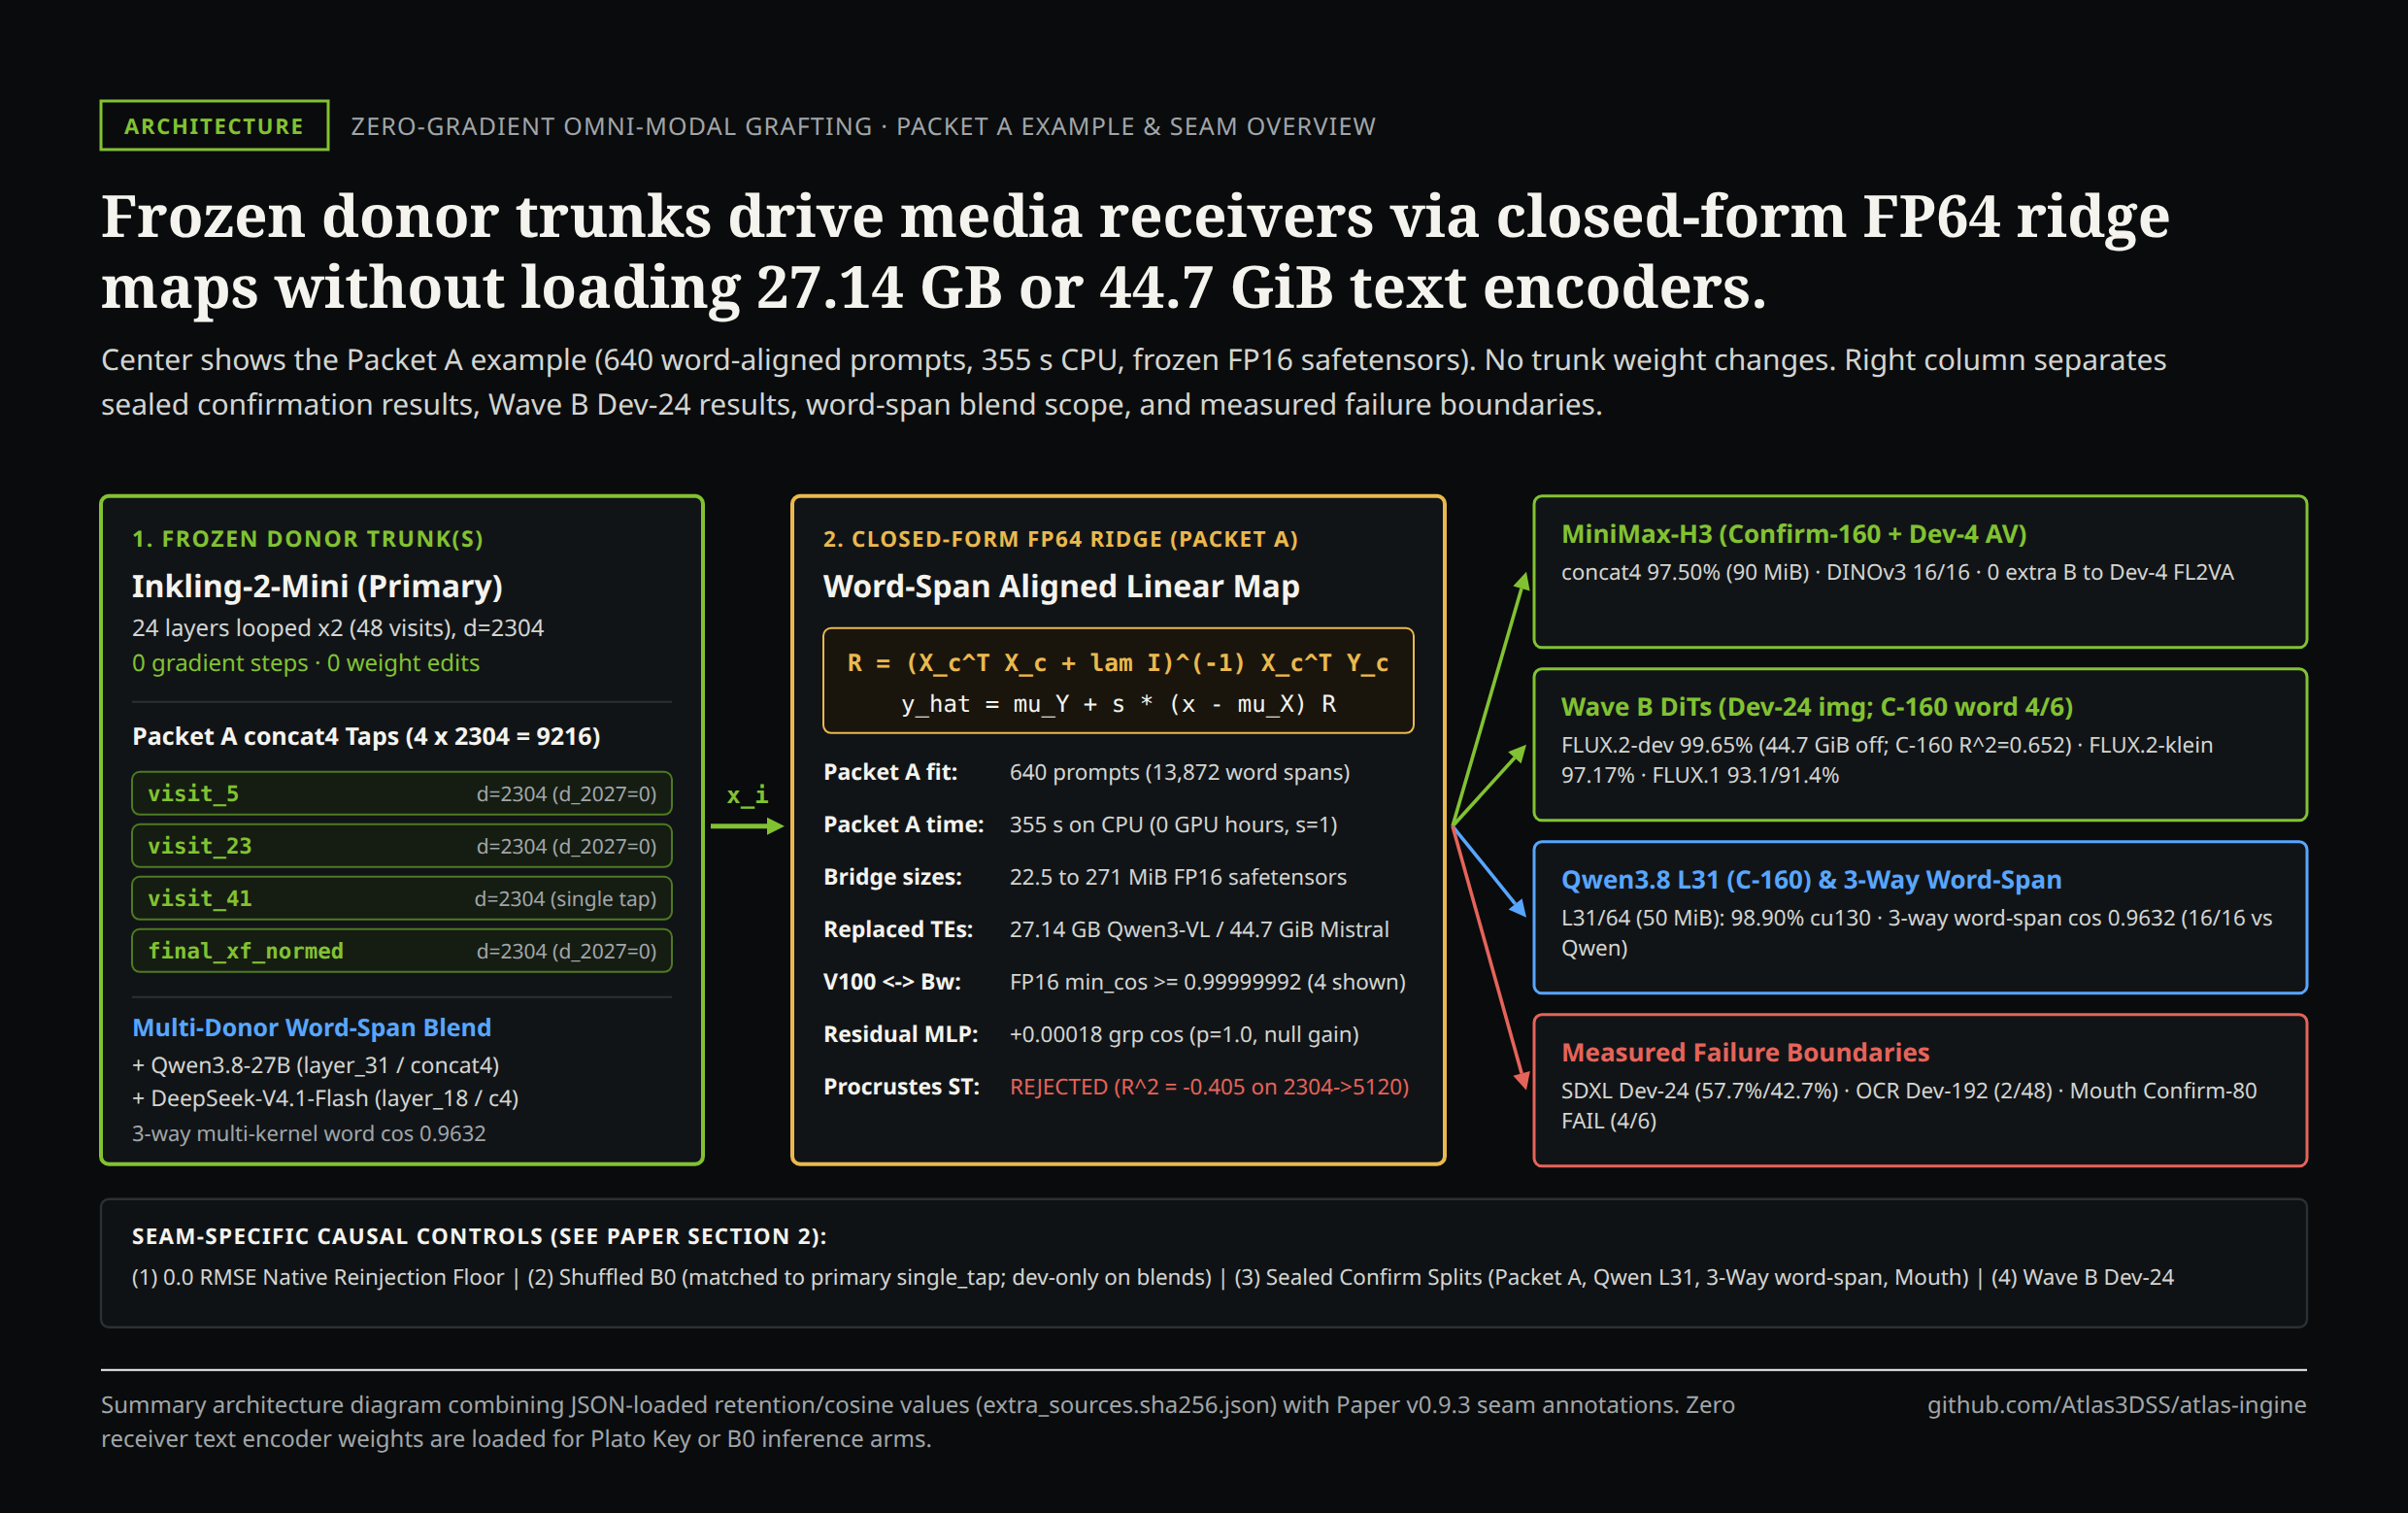
\includegraphics[width=0.96\textwidth,height=0.35\textheight,keepaspectratio]{figures/fig0_architecture_pipeline.png}
\caption{Zero-gradient omni-modal grafting overview. Frozen trunk activations map via FP64 closed-form ridge regression (Plato's Keys, $1.4\text{--}271\,\text{MiB}$ FP16 single-donor; up to $490\,\text{MiB}$ full-rank for 3-way blends) into image, video+audio, music, and speech receivers with zero trunk weight edits.}
\label{fig:arch}
\end{figure*}

\section{Method: Centered FP64 Ridge Mapping}
Given aligned source activations $X \in \mathbb{R}^{N \times d_s}$ (single layer or $4$-tap \texttt{concat4}) and target embeddings $Y \in \mathbb{R}^{N \times d_t}$ over $N$ word-aligned spans from $640$ training prompts ($N=13{,}872$ for Packet~A), we center both sides by fit-split means $\mu_X, \mu_Y$ ($X_c = X - \mathbf{1}\mu_X^\top$, $Y_c = Y - \mathbf{1}\mu_Y^\top$) and solve the exact FP64 regularized normal equations:
\begin{equation}
R^\star = (X_c^\top X_c + \lambda I)^{-1} X_c^\top Y_c, \qquad \hat{y} = \mu_Y + s\,(x - \mu_X) R^\star,
\end{equation}
where $\lambda$ and optional fit-only variance scale $s$ (default $s=1$) are selected strictly by source-group-disjoint inner cross-validation (never touching \texttt{val\_dev} or \texttt{confirm\_reserve}). Because \texttt{Qwen3-VL-32B} layer-50 states carry large anisotropic channel scales ($\text{RMS}\approx 47$), global $R^2$ remains high even under modest directional alignment (e.g.\ $R^2=0.8637$ on shuffled $B_0$ vs.\ $\cos=0.6425$); we therefore report word cosine alongside $R^2$ and downstream render metrics. On the matched single-tap inner comparison ($2304 \to 5120$), Orthogonal Procrustes fails ($R^2 = -0.405$) whereas centered ridge achieves $R^2 = +0.9948$ (and \texttt{concat4} reaches $R^2 = +0.9982$ on Confirm-160).

For $M$-donor blends ($X_c = [\sqrt{\alpha_1} X_{c,1}, \dots, \sqrt{\alpha_M} X_{c,M}]$), unweighted concatenation degrades at $M \ge 2$ due to inter-donor variance imbalance. \emph{Block-weighted multi-kernel ridge} allocates simplex weights $\alpha_m$ via inner-fold OOF MSE, scaling monotonically from $M=1 \to 2 \to 3$.

\section{Packet A: Sealed Image \& Video+Audio Transfer}
\subsection{Sealed Confirm-160 Image Evaluation (\texorpdfstring{$640$}{640} PNGs)}
Table~\ref{tab:packeta} reports the sealed $160$-prompt confirmation evaluation ($G=16$ disjoint source groups, $8$ domains, $4$ arms $= 640$ $1024\times 1024$ \texttt{MiniMax-H3} 6-step renders, $\texttt{fit\_calls}=0$, $4/4$ dev-floor reinject parity at $0.0$ RMSE; multi-arm Stage~B fit/selection elapsed $355.4\,\text{s}$ CPU in \texttt{stageB\_handoff\_manifest.json}). We define $B_0$-anchored H3 margin retention as $100\cdot(\text{cand}-B_0)/(\text{teacher}-B_0)$. Because shuffled $B_0$ is dimension-matched to the primary $2{,}304$-d \texttt{single\_tap} ($22.5\,\text{MiB}$) rather than $9{,}216$-d \texttt{concat4} ($90.0\,\text{MiB}$), \texttt{single\_tap} ($80.02\%$, $16/16$ groups vs.\ matched $B_0$, $p=3.05\times 10^{-5}$) is the primary matched-$B_0$ confirmation while \texttt{concat4} ($0.1982$ vs.\ $0.2045$ teacher, $\Delta=-0.0063$, 95\% CI $[-0.0117,-0.0010]$, descriptive $97.50\%$ vs.\ \texttt{single\_tap} $B_0$, $16/16$ over \texttt{single\_tap}, $p=3.05\times 10^{-5}$) is analyzed in its own block (Fig.~\ref{fig:packeta}).

\begin{table}[h]
\centering
\caption{Packet~A Sealed Confirm-160 ($640$ $1024\times 1024$ PNGs, $G=16$ groups, $0$ refits; SigLIP2 \cite{tschannen2025siglip2}).}
\label{tab:packeta}
\scriptsize
\setlength{\tabcolsep}{3.0pt}
\begin{tabular}{@{}lrrrr@{}}
\toprule
Arm (FP16 Size) & Word Cos & SigLIP2 & Margin & Img-Tch \\
\midrule
Teacher ($27.14\,\text{GB}$) & 1.0000 & \textbf{0.2045} & 100.0\% & 1.0000 \\
\texttt{concat4} ($90.0\,\text{MiB}$)$^\dagger$ & \textbf{0.9228} & \textbf{0.1982} & \textbf{97.5\%}$^\dagger$ & \textbf{0.8942} \\
\texttt{single\_tap} ($22.5\,\text{MiB}$) & 0.7961 & 0.1544 & 80.0\% & 0.7669 \\
Shuffled $B_0$ ($22.5\,\text{MiB}$) & 0.6425 & $-0.0463$ & 0.0\% & 0.4873 \\
\bottomrule
\multicolumn{5}{@{}l@{}}{\tiny $^\dagger$Separate analysis block; $B_0$ is dimension-matched to \texttt{single\_tap} ($2304$-d).}
\end{tabular}
\end{table}

\begin{figure*}[t]
\centering
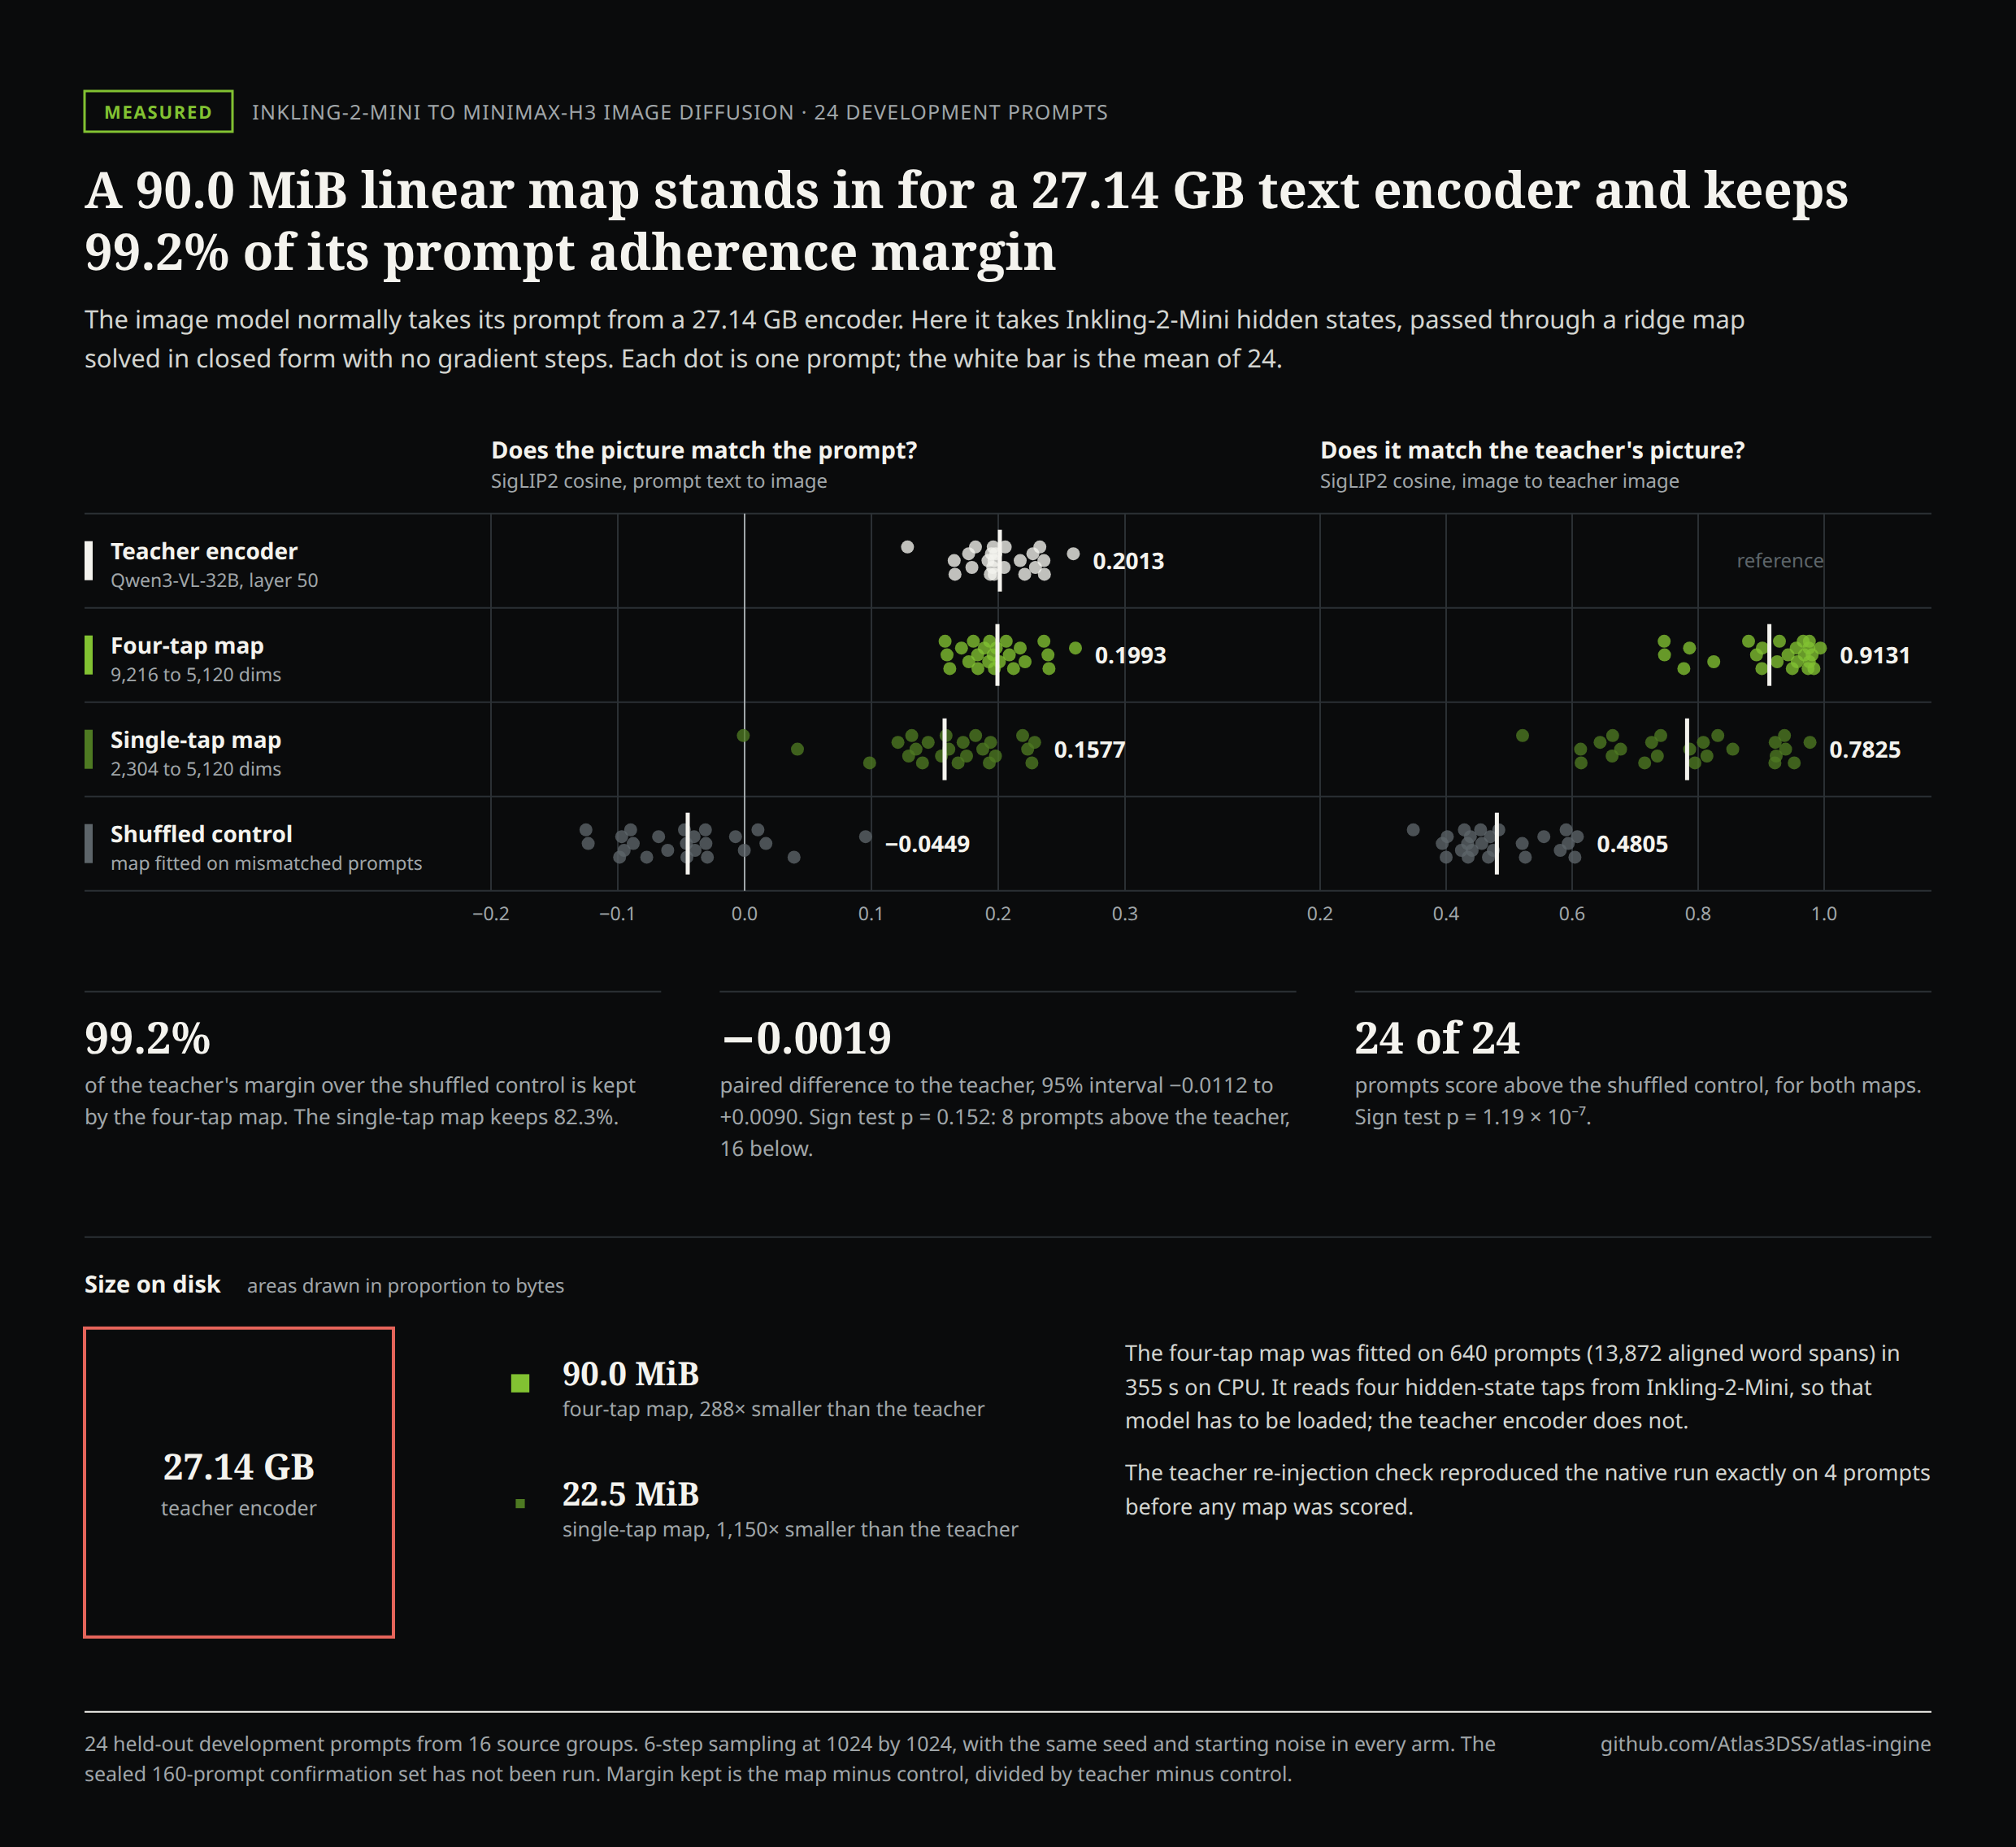
\includegraphics[width=0.90\textwidth,height=0.40\textheight,keepaspectratio]{figures/fig1_packetA_adherence_and_size.png}
\caption{Packet~A Sealed Confirm-160 SigLIP2 prompt-to-image adherence, image-to-teacher cosine, and disk compression ($27.14\,\text{GB} \to 90.0\,\text{MiB}$ \texttt{concat4} / $22.5\,\text{MiB}$ \texttt{single\_tap}) across $640$ rendered PNGs.}
\label{fig:packeta}
\end{figure*}

\subsection{Orthogonal DINOv3 Teacher Similarity \& MLP Baseline}
Scoring the same $640$ Confirm-160 PNGs with self-supervised \texttt{DINOv3-ViT-L/16} \cite{simeoni2025dinov3} measures image-to-teacher feature similarity (not independent prompt adherence): \texttt{concat4} beats both \texttt{single\_tap} and $B_0$ on $16/16$ groups ($p=3.05\times 10^{-5}$; CLS $0.7599\pm 0.1041$ vs.\ $0.4871$/$0.0309$, mean-patch $0.8697\pm 0.0592$, spatial patch-to-patch $0.6910\pm 0.1083$ vs.\ $0.1729$ $B_0$).

On identical $640$-prompt word-span data ($13{,}872$ spans, fold-0 inner selection, report \texttt{fab778e4}), a gradient-trained \texttt{ResidualRidgeMLP} ($76.56\,\text{M}$ total params, $29.37\,\text{M}$ residual branch, $146.0\,\text{MiB}$ FP16, initialized at exact ridge) yielded no statistically detectable grouped word-span cosine gain on Confirm-160 ($\Delta=+0.00018$, exact $+0.0001759$, 95\% CI $[-0.00074,+0.00115]$, $8/16$ groups, $p=1.0$), while a scratch 2-layer GELU MLP ($40$ epochs) reached $R^2=0.505$.

\subsection{Zero-Refit Video+Audio \& Separately Fitted DiT Receivers}
Only H3 image $\to$ \texttt{FL2VA} video+audio reused the exact identical $90.0\,\text{MiB}$ \texttt{concat4} bytes (\texttt{cca1e5bc}, zero refit): $4$-prompt paired quality audits ran at $56$ frames, while hardware demonstrations rendered $141$-frame ($5.875\,\text{s}$) $768\times 448$ video + $32\,\text{kHz}$ stereo audio across $16$ distinct GPUs (Section~\ref{sec:silicon}).

Separately fitted keys against external DiT text encoders (Blackwell \texttt{sm\_120}, zero upstream text encoder loaded) are evaluated on Dev-24 renders using external retention $100\cdot\text{cand\_margin}/\text{native\_margin}$ with a separate shuffled-$B_0$ sign-test gate (not directly comparable to H3 $B_0$-anchored retention):
\begin{itemize}[leftmargin=1.2em,itemsep=1.5pt]
\item \textbf{Wave A (Dev-24 renders, Turbo / Base):} \texttt{Z-Image} $98.88\%$ Turbo / $101.19\%$ Base ($45.1\,\text{MiB}$); \texttt{FLUX.2-klein-4B} $97.73\%$ Turbo / $83.49\%$ Base ($135.2\,\text{MiB}$); \texttt{Qwen-Image-2.1} $96.37\%$ Turbo / $98.80\%$ Base ($16.33\,\text{GB}$ peak); \texttt{FLUX.3-Image-Klein} $97.33\%$ Turbo / $99.02\%$ Base ($12.0\,\text{GB}$ peak).
\item \textbf{Wave B (Dev-24 renders + $6/6$ Confirm-160 word bars; Confirm-160 image renders sealed):} Across all $6$ Wave~B targets on sealed Confirm-160 word spans ($160$ prompts, $3{,}413$ rows, summary \texttt{1b712f15}), $4/6$ targets passed the $R^2\ge 0.55$ word bar ($4/4$ decoder-LLM targets): \texttt{FLUX.2-dev} passed one-shot Confirm-160 word alignment ($\cos=0.878041$, $R^2=0.652314$, $16/16$ positive group $\Delta R^2$ vs.\ $B_0$, CI $[0.8757,0.9527]$, report \texttt{bb253f5d}; Dev-24 render $99.65\%$ replacing $44.7\,\text{GiB}$ Mistral-24B with a $271\,\text{MiB}$ key), alongside \texttt{p\_image\_oss} (Dev-24 $99.09\%$, C-160 word $\cos=0.9746$, $R^2=0.8449$), \texttt{FLUX.2-klein-9B} (Dev-24 Base $97.17\%$, C-160 word $\cos=0.9426$, $R^2=0.7197$), and \texttt{moss\_image} (Dev-24 $98.25\%/95.38\%$, C-160 word $\cos=0.9191$, $R^2=0.6869$). Two targets missed the word bar: \texttt{FLUX.1-dev/schnell} (Dev-24 $93.07\%/91.44\%$, C-160 word $R^2=0.5296 < 0.55$) and \texttt{SDXL} (Dev-24 FAIL $57.69\%$ Base / $42.66\%$ Turbo, C-160 word $R^2=0.5403$; unmasked 77-token \texttt{CLIP-L} padding dilution is a mechanistic hypothesis without an isolating ablation).
\end{itemize}

\section{Failure Boundaries: Vision OCR \& Speech}
\begin{enumerate}[leftmargin=1.2em,itemsep=2pt]
\item \textbf{Reverse Vision$\to$LLM OCR (Packet~B/B2, dev-only):} In Packet~B ($72/192$ overall agree; Fig.~\ref{fig:ocr}), frozen ridge into \texttt{Inkling-2-Mini} \texttt{EmbedRows} achieves $45/48$ teacher agreement ($40/48$ gold) on counting/layout, while typography fails ($1\to 3/48$ agree, $1\to 2/48$ gold under rejected \texttt{ridge\_norm}). Under Packet~B2 high-res masked towers (evaluated against its re-pinned $64/192$ comparator with $38/48$ counting), counting stayed $38\to 38/48$, charts moved $1\to 8/48$ agreement ($2/48$ gold), typography remained $1\to 2/48$ agreement ($1\to 0/48$ gold), and overall gold was $62\to 63/192$ ($p=1.0$, $2/5$ dev gates; locked $448$-item test remains $0$ touched).
\item \textbf{Speech Lexemes \& One-Shot Mouth Confirm (Packet~C):} Direct continuous lexical projection failed $0/32$ pairs on dev. Supplying discrete text tokens in hybrid confirm ($80$ items, $400$ WAVs) held $29/32$ supplied-text lexical accuracy and passed $4/6$ amended gates, but failed both style gates ($21/32 < 22$ bar; $21/32$ vs.\ $11/32$ swapped, $p=0.110184$) due to a frozen-scorer intonation inversion ($0/8$ vs.\ $8/8$). Speech perception (Ears) remains $0/80$ sealed on confirm (dev-only pace/nonspeech checks).
\end{enumerate}

\begin{figure*}[t]
\centering
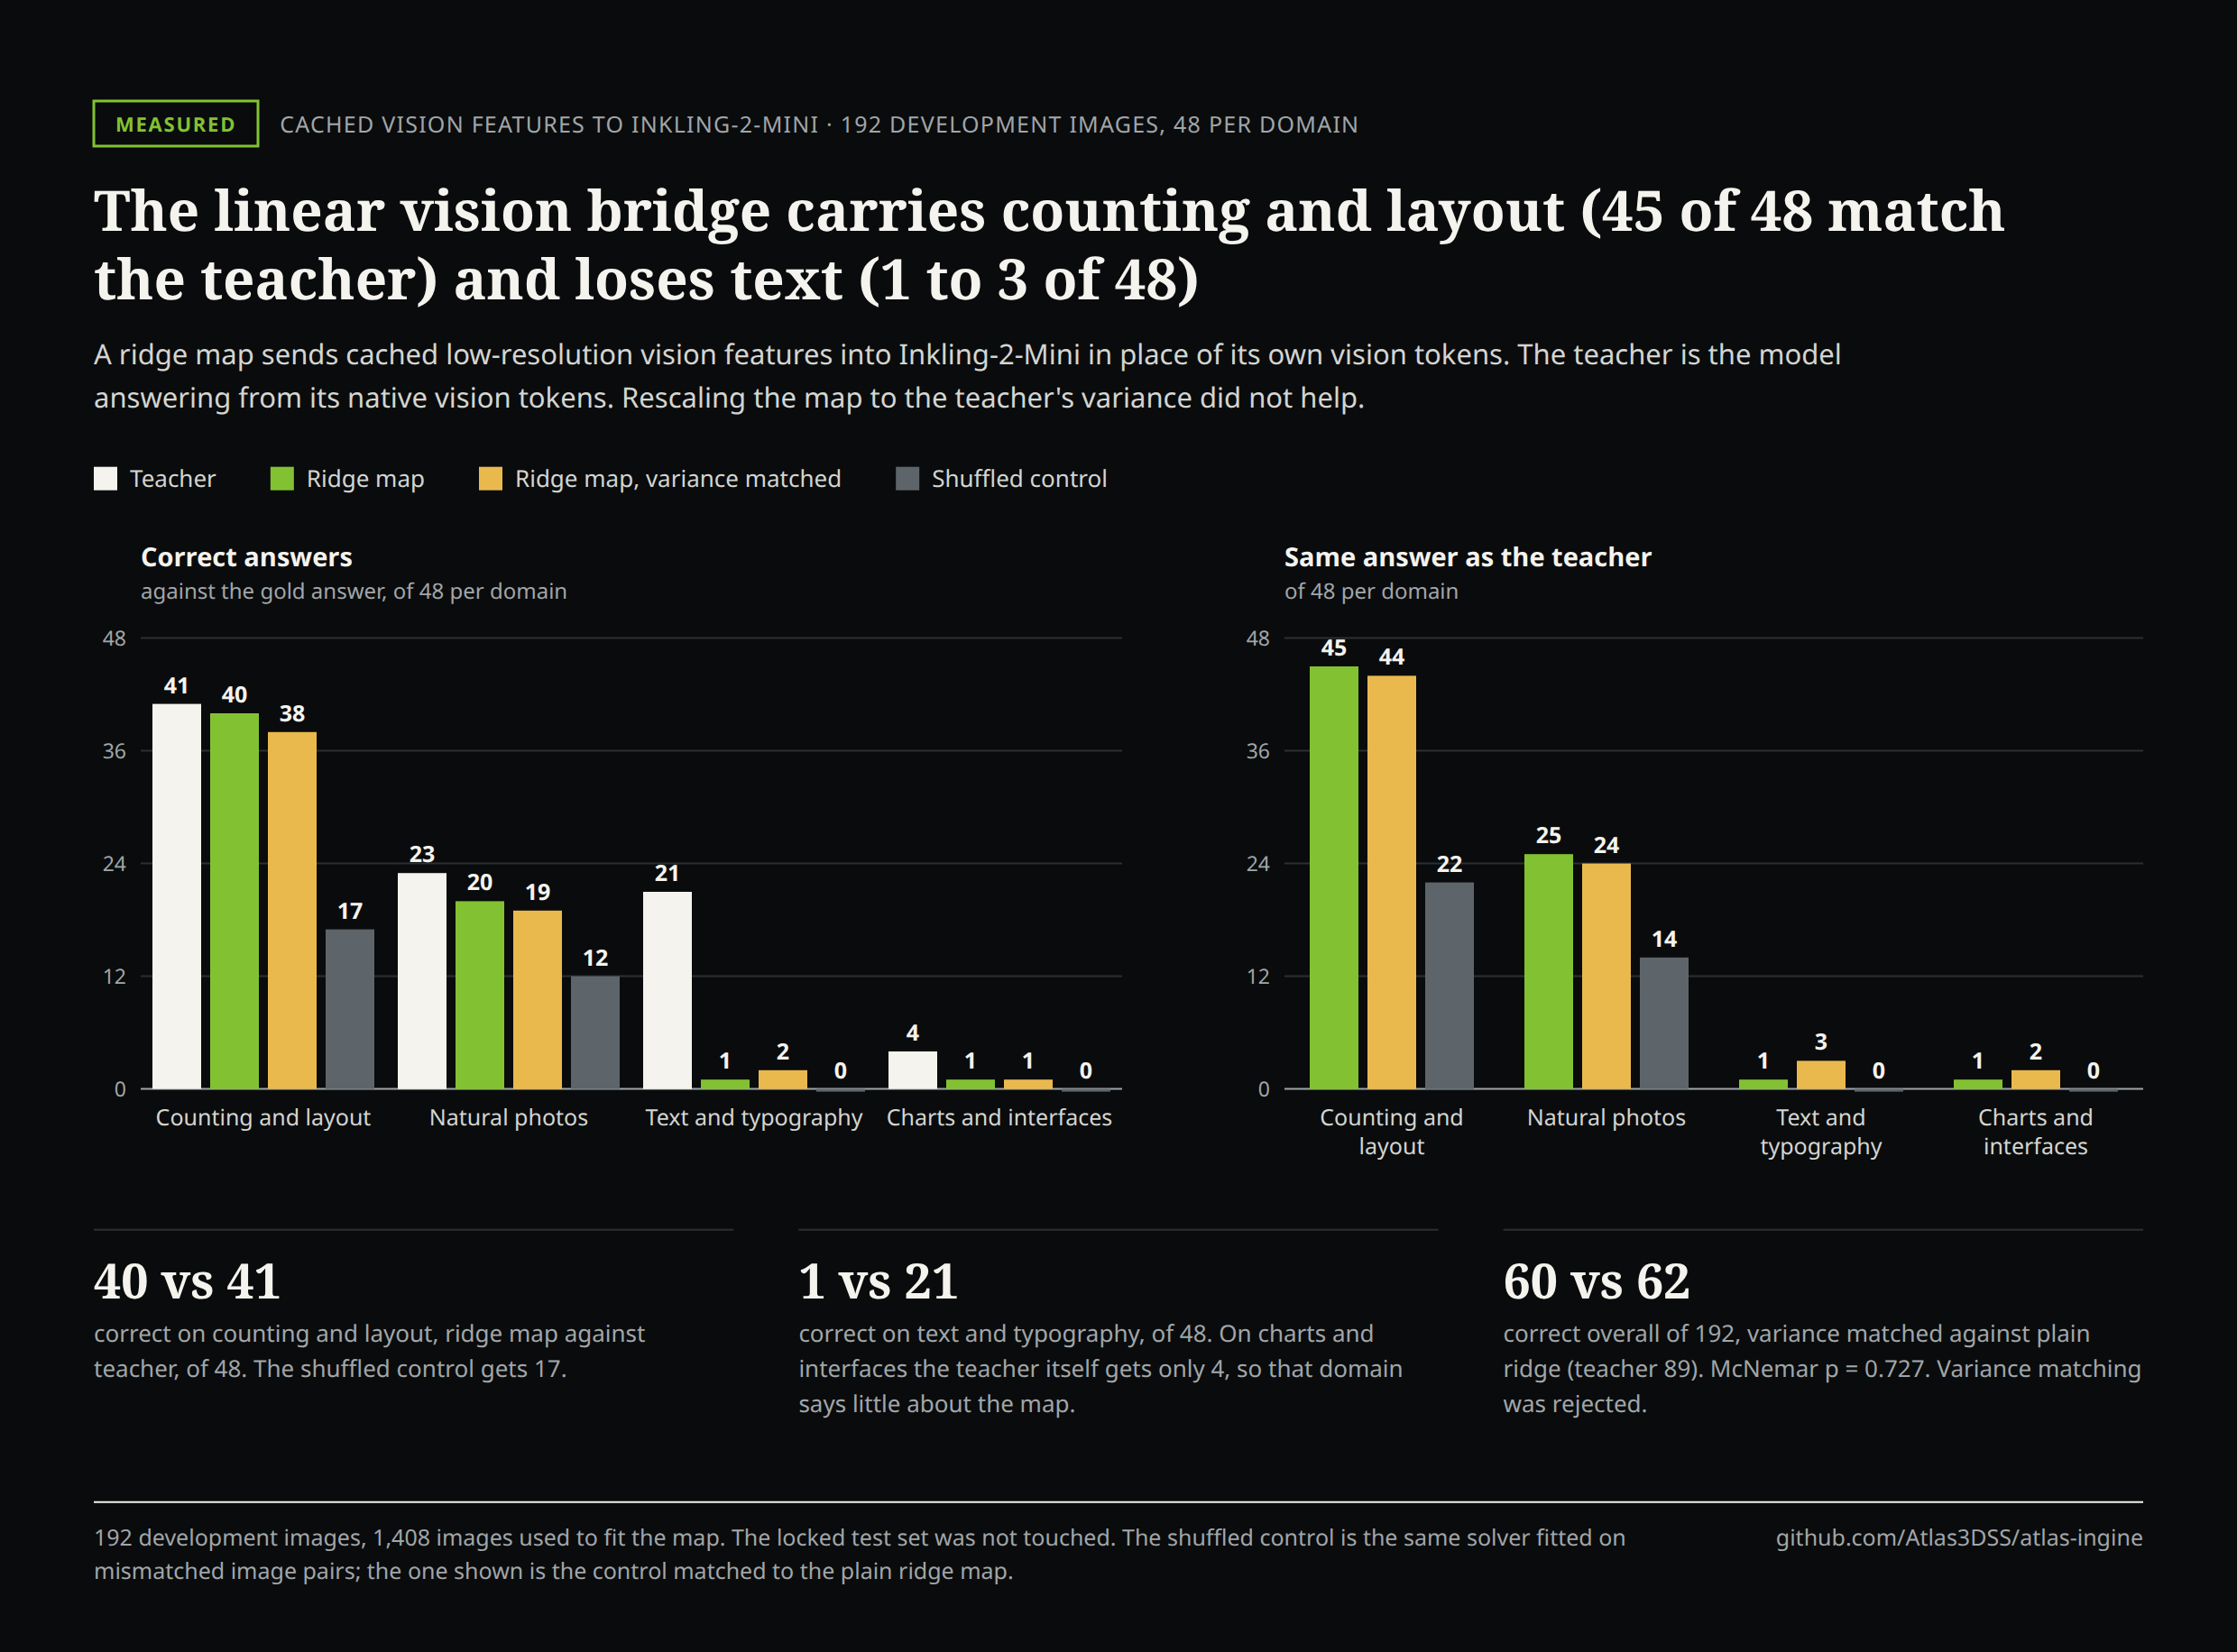
\includegraphics[width=0.90\textwidth,height=0.35\textheight,keepaspectratio]{figures/fig2_packetB_ocr_boundary.png}
\caption{Packet~B Vision$\to$LLM linear boundary on $192$ development images ($48$/domain; $448$-item locked test untouched): counting/layout transfers ($45/48$ agree, $40/48$ gold), while typography fails under both \texttt{ridge\_frozen} ($1/48$) and rejected \texttt{ridge\_norm} ($3/48$ agree, $2/48$ gold). Packet~B2 high-res tower ablations are reported in text.}
\label{fig:ocr}
\end{figure*}

\section{Multi-Donor Blends, Spectral Rank, MoE Sparsity, \& Prosody}
\subsection{Multi-Donor Blends \& Half-Depth \texorpdfstring{\texttt{Qwen3.8}}{Qwen3.8} L31}
Across $3$ real donor families (\texttt{Qwen3.8-27B}, \texttt{Inkling-2-Mini}, \texttt{DeepSeek-V4.1-Flash}) on sealed Confirm-160 word spans ($n=3{,}413$ words, $G=16$ groups; no blend renders), unweighted stacking controls ($0.9585, 0.9569, 0.9566$) fall below Confirm-$R^2$-selected single \texttt{Qwen3.8} ($0.9596$), whereas block-weighted \texttt{stacked\_multikernel\_concat4} reaches $0.963201$ pooled word cosine ($+0.003602$ equal-group paired vs.\ \texttt{Qwen3.8}, $16/16$ groups, $p=3.05\times 10^{-5}$; $8/8$ domains and $+0.000601$ vs.\ 2-way descriptive; shuffled controls dev-only; Fig.~\ref{fig:multidonor}).

In controlled same-host \texttt{PRO 6000 cu130} Confirm-160 renders ($640$ images), a \emph{separately fitted} \texttt{Qwen3.8-27B} half-depth key (\texttt{layer\_31/64}, $50.02\,\text{MiB}$) passes matched-$B_0$ ($16/16$, $p=3.05\times 10^{-5}$, $B_0=-0.057508$) with $98.90\%$ retention ($0.201639$ vs.\ $0.204513$ teacher, $\Delta=-0.002874$, 95\% CI $[-0.00694,+0.00147]$; neither equivalence nor end-to-end speedup tested).

\begin{figure*}[t]
\centering
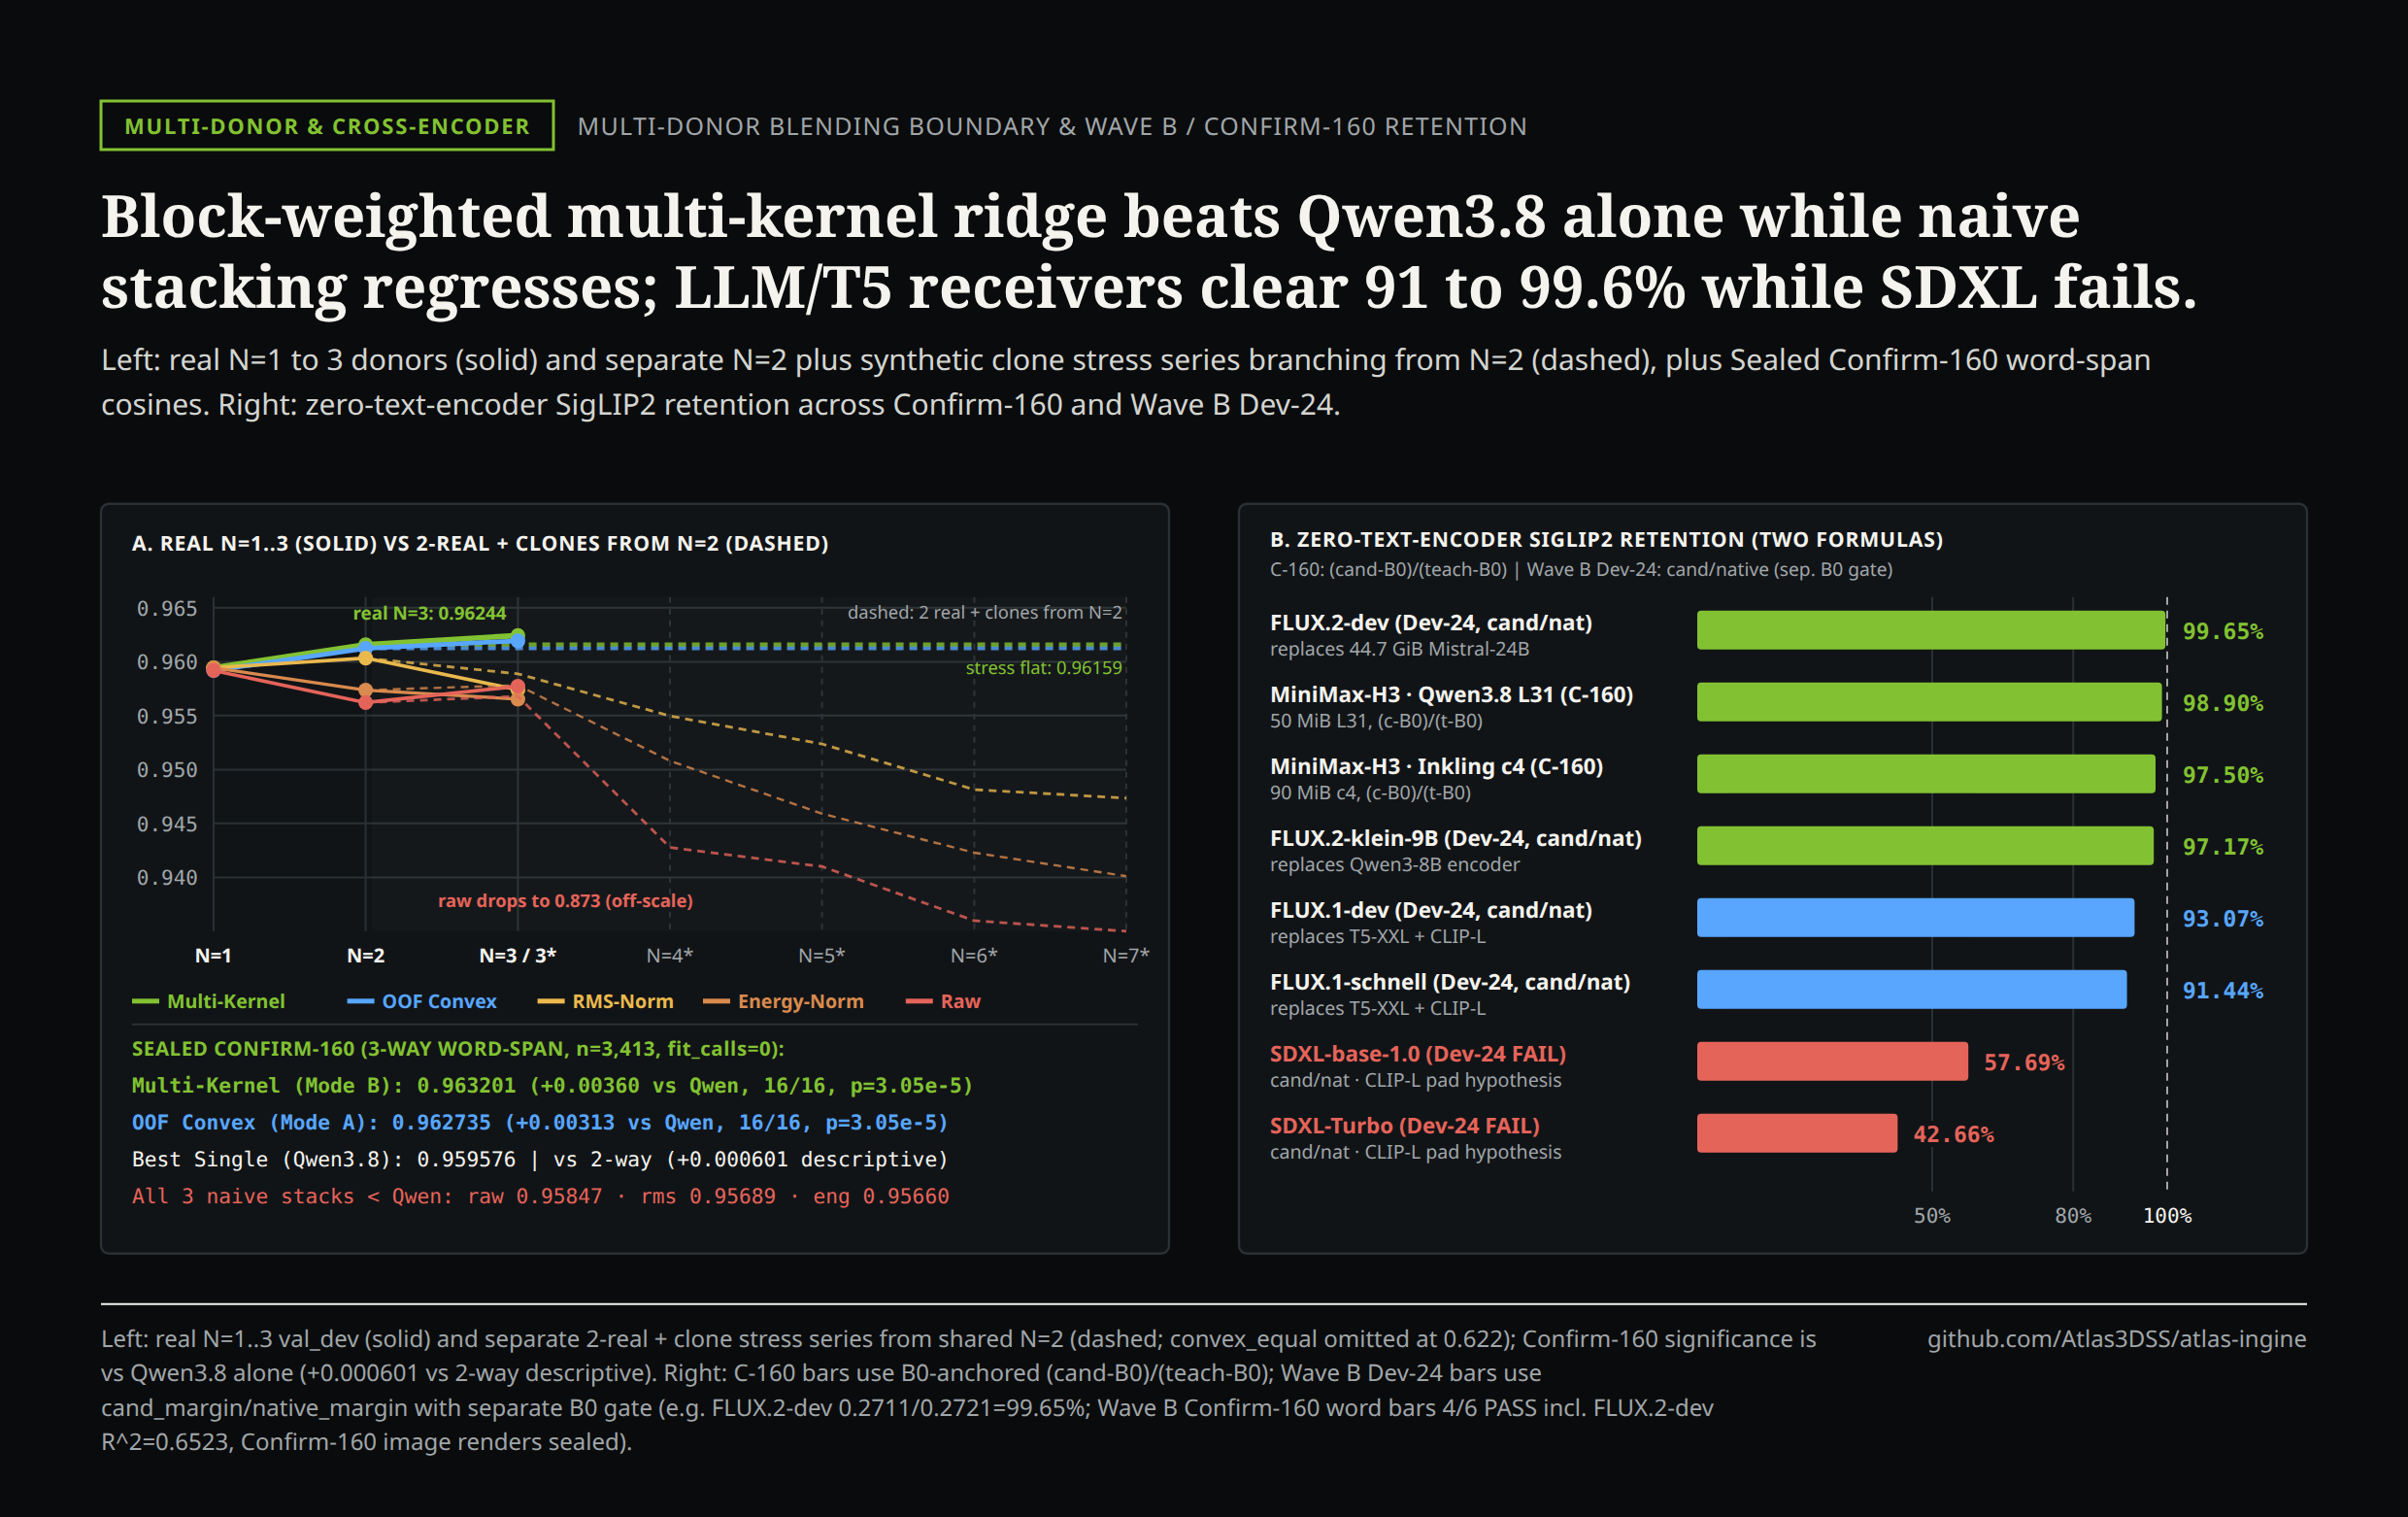
\includegraphics[width=0.95\textwidth,height=0.36\textheight,keepaspectratio]{figures/fig4_multidonor_and_universal.png}
\caption{Left: Multi-donor word-span scaling ($N=1\to 3$ real donors vs.\ synthetic clones) and Confirm-160 3-way results. Right: H3 $B_0$-anchored retention (Confirm-160) beside separately defined Wave~B Dev-24 external retention (not pooled across formulas; Wave~B Confirm-160 word bars $4/6$ PASS, image renders sealed).}
\label{fig:multidonor}
\end{figure*}

\subsection{FP64 Spectral Rank \& Live V100 MoE Pruning}
Exact FP64 SVD of $20$ fitted keys evaluated on strictly held-out \texttt{val\_dev} ($\texttt{confirm\_reserve\_touched}=0$, \texttt{7aff2432}; sizes are FP16 low-rank factor estimates without timed render validation yet; Fig.~\ref{fig:svd_prosody}A--B) shows sharp modality-specific compressibility:
\begin{itemize}[leftmargin=1.2em,itemsep=1.5pt]
\item \textbf{Speech/Mouth keys:} \texttt{Inkling} ($26.2\times$, $1.4\,\text{MiB}$, $r_{\text{eff}}=51.0$) and \texttt{DeepSeek-V4.1} ($29.1\times$, $2.8\,\text{MiB}$) text heads compress at $r=64$ ($<0.001$ cos loss), whereas \texttt{Qwen3.8} text and instruct heads require $r=192$ ($9.7\times$, $8.2\,\text{MiB}$); \texttt{Inkling}/\texttt{DeepSeek} instruct heads compress $13.1\times/14.5\times$ at $r=128$.
\item \textbf{Video H3 \& Image DiT keys:} H3 \texttt{concat4} keys hit the $-0.002$ cosine knee at $2.1\times\text{--}7.6\times$ ($21\text{--}75\,\text{MiB}$; single taps down to $1.0\times$; 3-way multikernel $r=2048$ takes $216\,\text{MiB}$ vs.\ $490\,\text{MiB}$ full; \texttt{FLUX.2-dev} evaluated against full-rank surrogate predictions). Normalized tap output contribution ($\%Y$) peaks at mid-depth for \texttt{Qwen3.8} (\texttt{layer\_31}$=95.8\%$), \texttt{Inkling} (\texttt{visit\_23}$=66.5\%$), and \texttt{GLM-5.3} (\texttt{layer\_21}$=67.1\%$), and late-mid for \texttt{DeepSeek-V4.1} (\texttt{layer\_33}$=63.2\%$).
\item \textbf{Live V100 MoE specialization \& donor-prefill cold-expert pruning (\texttt{val\_dev} word-span only, \texttt{fb8db8f0}):} Across $24$ physical layers $\times 128$ experts (top-8) on \texttt{Inkling-2-Mini} ($n=3{,}446$ \texttt{val\_dev} words, $0$ confirm, $0$ DiT renders), Media vs.\ Code/Math routing cosine is $0.3926$ vs.\ $0.99812$ within Media ($142\times$ higher JS divergence, $0.3794$ vs.\ $0.00266$ bits; $32.5/128$ experts cover $80\%$ of Media mass). Fit-ranked live V100 pruning removes $\mathbf{60\%}$ of cold experts ($51/128$ surviving) for a $\mathbf{1.71\times}$ donor prompt-prefill speedup ($497.1 \to 290.6\,\text{ms/prompt}$, excluding diffusion) at $-0.00400$ \texttt{val\_dev} cosine on \texttt{hf\_native\_concat4} ($0.92015 \to 0.91616$; the frozen NVFP4 Packet~A key on the same HF V100 trunk shifts $0.87454 \to 0.87004$ due to BF16/NVFP4 exporter mismatch), while pass-1 early exit (\texttt{exit\_pass1\_v29}, $62.5\%$ FLOPs) retains $0.91185$ ($-0.00830$).
\end{itemize}

\subsection{5-Family Expressive Open-Source TTS Shoot-Out}
Across a $1{,}416$-clip anonymized corpus (including human anchors and \texttt{YuE2} singing; report \texttt{72ae01e0}; $256$ cross-shard comparisons of human recordings verify frozen-judge reproducibility at $\max|\Delta\text{WER}|=0.0$, $\max|\Delta p|=0.001488$, not human ratings), the primary 5-family TTS comparison spans $60$ matched texts ($40$ RAVDESS + $20$ EmergentTTS) under frozen \texttt{emotion2vec+} and \texttt{faster-whisper} gated by $\text{RMS}\ge 0.01$ (Fig.~\ref{fig:svd_prosody}C):
\begin{itemize}[leftmargin=1.2em,itemsep=1.5pt]
\item \textbf{\texttt{Qwen3-TTS} + \texttt{Qwen3.8} Plato's Key continuous style} reached $24/60$ ($40.0\%$) \texttt{e2v+} top-1 vs.\ $26/60$ ($43.3\%$) native hand-written ceiling ($-3.3\,\text{pp}$, $6$ improved / $8$ regressed, paired CI $[-15.0,+8.3]\,\text{pp}$, exact McNemar $p=0.79053$, supporting neither parity nor equivalence), cut $n=60$ WER from $33.91\% \to 23.18\%$ (Track~2 silence-gate pass-only WER $17.39\%$ on $48/60$ $\to 11.36\%$ on $52/60$; all-80 native ceiling pass-only $18.17\%$ on $68/80$), and showed the highest observed melancholic \texttt{sad} recall at $6/14$ ($42.9\%$) vs.\ $5/14$ \texttt{Orpheus-3B} (small-sample descriptive; no supported winner claim across 20 arms). Stock greedy \texttt{Qwen3-TTS} exhibited a $5.68\,\text{s}$ silence attractor on short 6-word RAVDESS prompts (on EmergentTTS, \texttt{armA\_simple\_tag} passed $39/40 = 97.5\%$, native ceiling $40/40$, and both Plato's Key continuous arms $20/20$ on their $20$-item EmergentTTS subset); sampled decoding + RMS retry is a proposed mitigation awaiting evaluation.
\item \textbf{Rival TTS \& singing:} \texttt{Orpheus-TTS-3B} (Apache-2.0) reached $18/60$ ($30.0\%$, $60/60$ above RMS threshold, $3.09\%$ WER); \texttt{Chatterbox-0.5B} ($15/60$, $1.42\%$ WER, retired Aug~2026) tested $1.000$ PerTh-watermarked on $10/10$ checked clips; \texttt{Step-Audio-EditX} reached $12/60$ ($-23.3\,\text{pp}$ vs.\ Qwen3 ceiling, $p=0.00434$); \texttt{IndexTTS-2} (non-commercial) had a happy-timbre bias ($0/14$ \texttt{sad}), yet 4-fold OOF Plato's Key vectors lifted RAVDESS-40 from $0/40$ to $6/40$ (nominal exploratory $p=0.03125$; overall $n=60$ was $7/60$ vs.\ $2/60$ native ceiling, exact McNemar $p=0.125$ n.s., and vs.\ $1/60$ neutral/swapped $p=0.0703$ n.s.). On \texttt{YuE2-3B} (CC-BY-NC-4.0), continuous Plato's Key affect matched symbolic tempo/key on $4/4$ songs ($78.5\,\text{BPM}$, \texttt{K:Bb} vs.\ $156.75\,\text{BPM}$ swapped; speech \texttt{e2v+} failed $0/12$ on accompanied music).
\end{itemize}

\begin{figure*}[t]
\centering
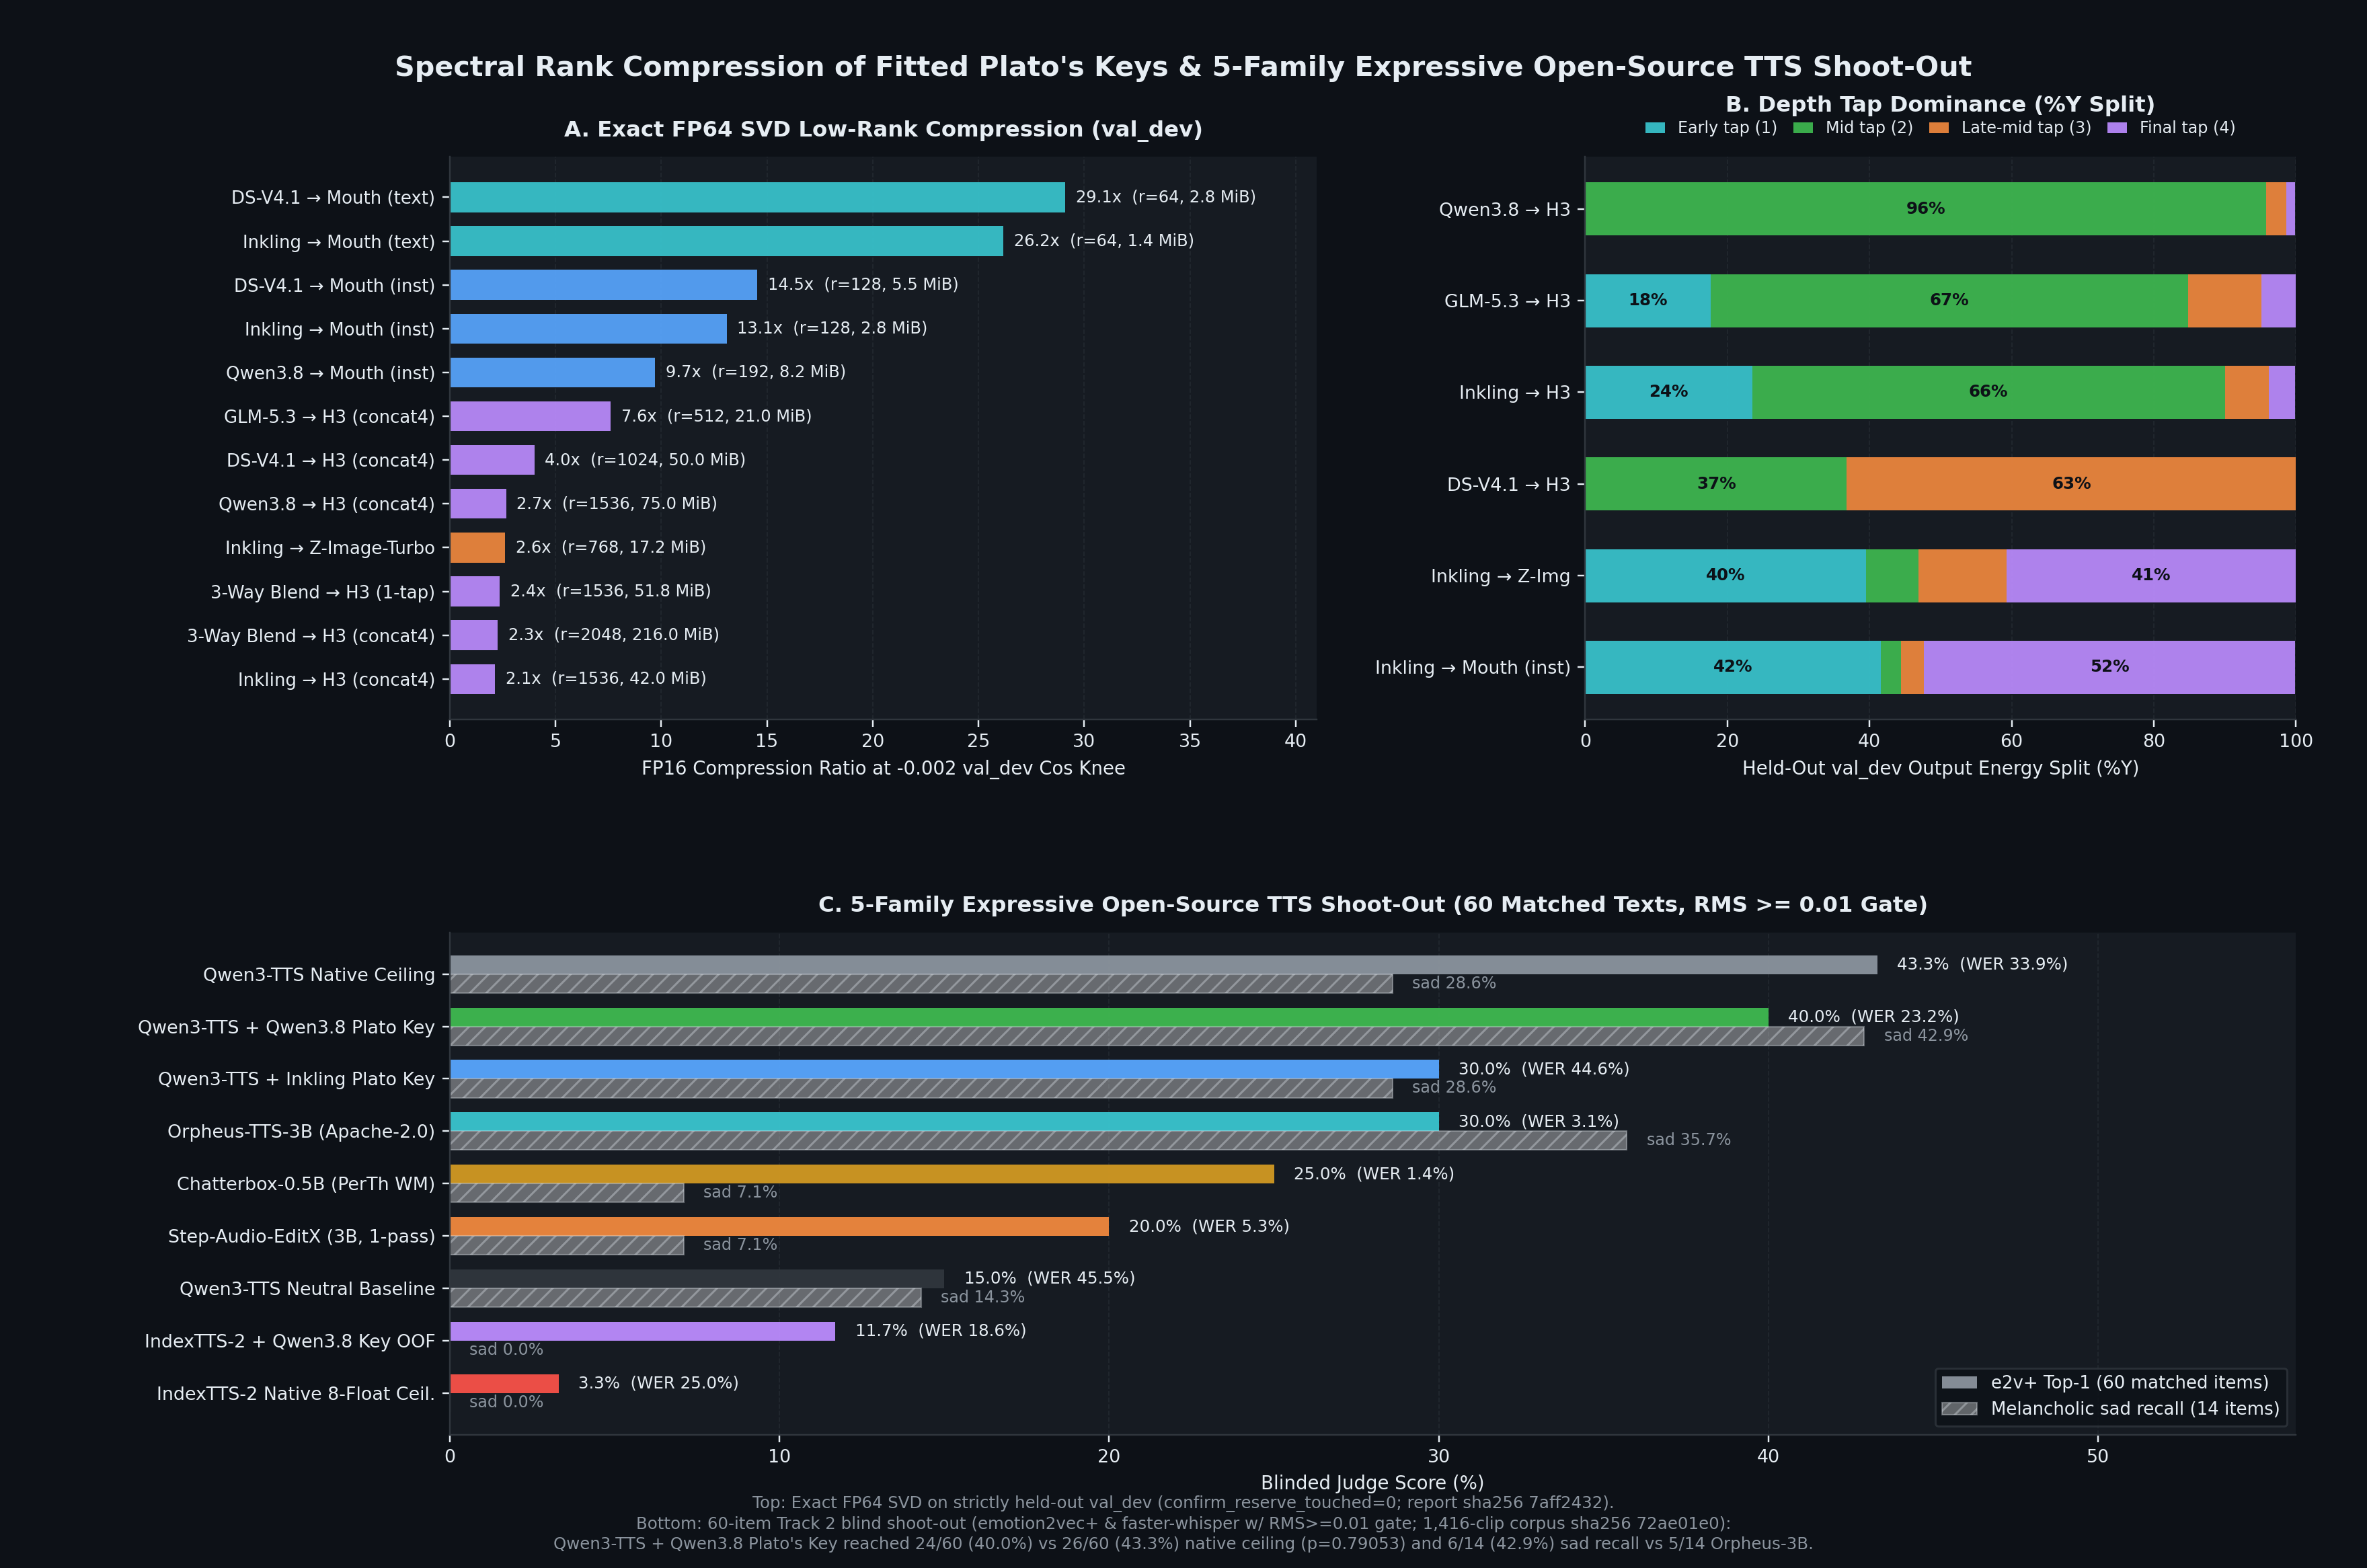
\includegraphics[width=0.95\textwidth,height=0.40\textheight,keepaspectratio]{figures/fig5_lowrank_svd_and_prosody.png}
\caption{(A) Exact FP64 SVD compression at the $-0.002$ \texttt{val\_dev} cosine knee (\texttt{7aff2432}). (B) Normalized held-out tap output contribution ($\%Y$). (C) 5-family expressive TTS shoot-out on $60$ matched texts (\texttt{72ae01e0}).}
\label{fig:svd_prosody}
\end{figure*}

\section{Host-Enforced Alignment \& Proposed \texorpdfstring{\texttt{LoopRes}}{LoopRes} Pilot}
On a single local model (\texttt{Inkling-2-Mini-atlas-12g}, \texttt{ingine-serve -\/-persona-probe-mode}) across $40$ sequential adversarial proposals spanning five instrumented invariants plus $10$ benign controls (Fig.~\ref{fig:closedloop}B, report \texttt{eb8b7923}): \textbf{Arm~A} (system-prompt constitution only) emitted $22/40$ ($55.0\%$) policy-violating proposals, whereas \textbf{Arm~B} (Host-Enforced Verified Ledger) committed $0/40$ ($0.0\%$) violations on those $40$ proposals while admitting $10/10$ ($100.0\%$) benign commits. Separate checks verified $3/3$ \texttt{HTTP 400} rejections on direct \texttt{/v1/probe/chat} $d=2027$ tampers and $50/50$ audited hash-chain events. Selected breached base64/hex IP traces exhibited larger live MoE routing shifts ($0.0375\text{--}0.0824$) than one refused direct comparator ($0.0081$, $n=1$ benign IP centroid; $3/5$ domains had $0$ tapped benign turns; exploratory telemetry, not a validated detector or population security guarantee).

\textbf{Proposed Gradient-Trained Pilot (Unmeasured):} Distinct from our measured zero-gradient grafts above, we propose integrating \texttt{LoopRes} \cite{zhao2026loopres} (MIT, \texttt{arXiv:2611.31094}) on \texttt{Qwen3-1.7B} only (\texttt{Qwen3.8} would require a separate follow-on protocol): deterministic Verified Ledger trajectories feed preregistered \texttt{LoopRes} SFT targeting reductions on context-observable adversarial attacks relative to matched stock SFT (seven canonical attacks depend on hidden host state), followed by Phase~2 closed-form H3 word-span re-lock (rendering optional; Fig.~\ref{fig:closedloop}A).

\begin{figure*}[t]
\centering
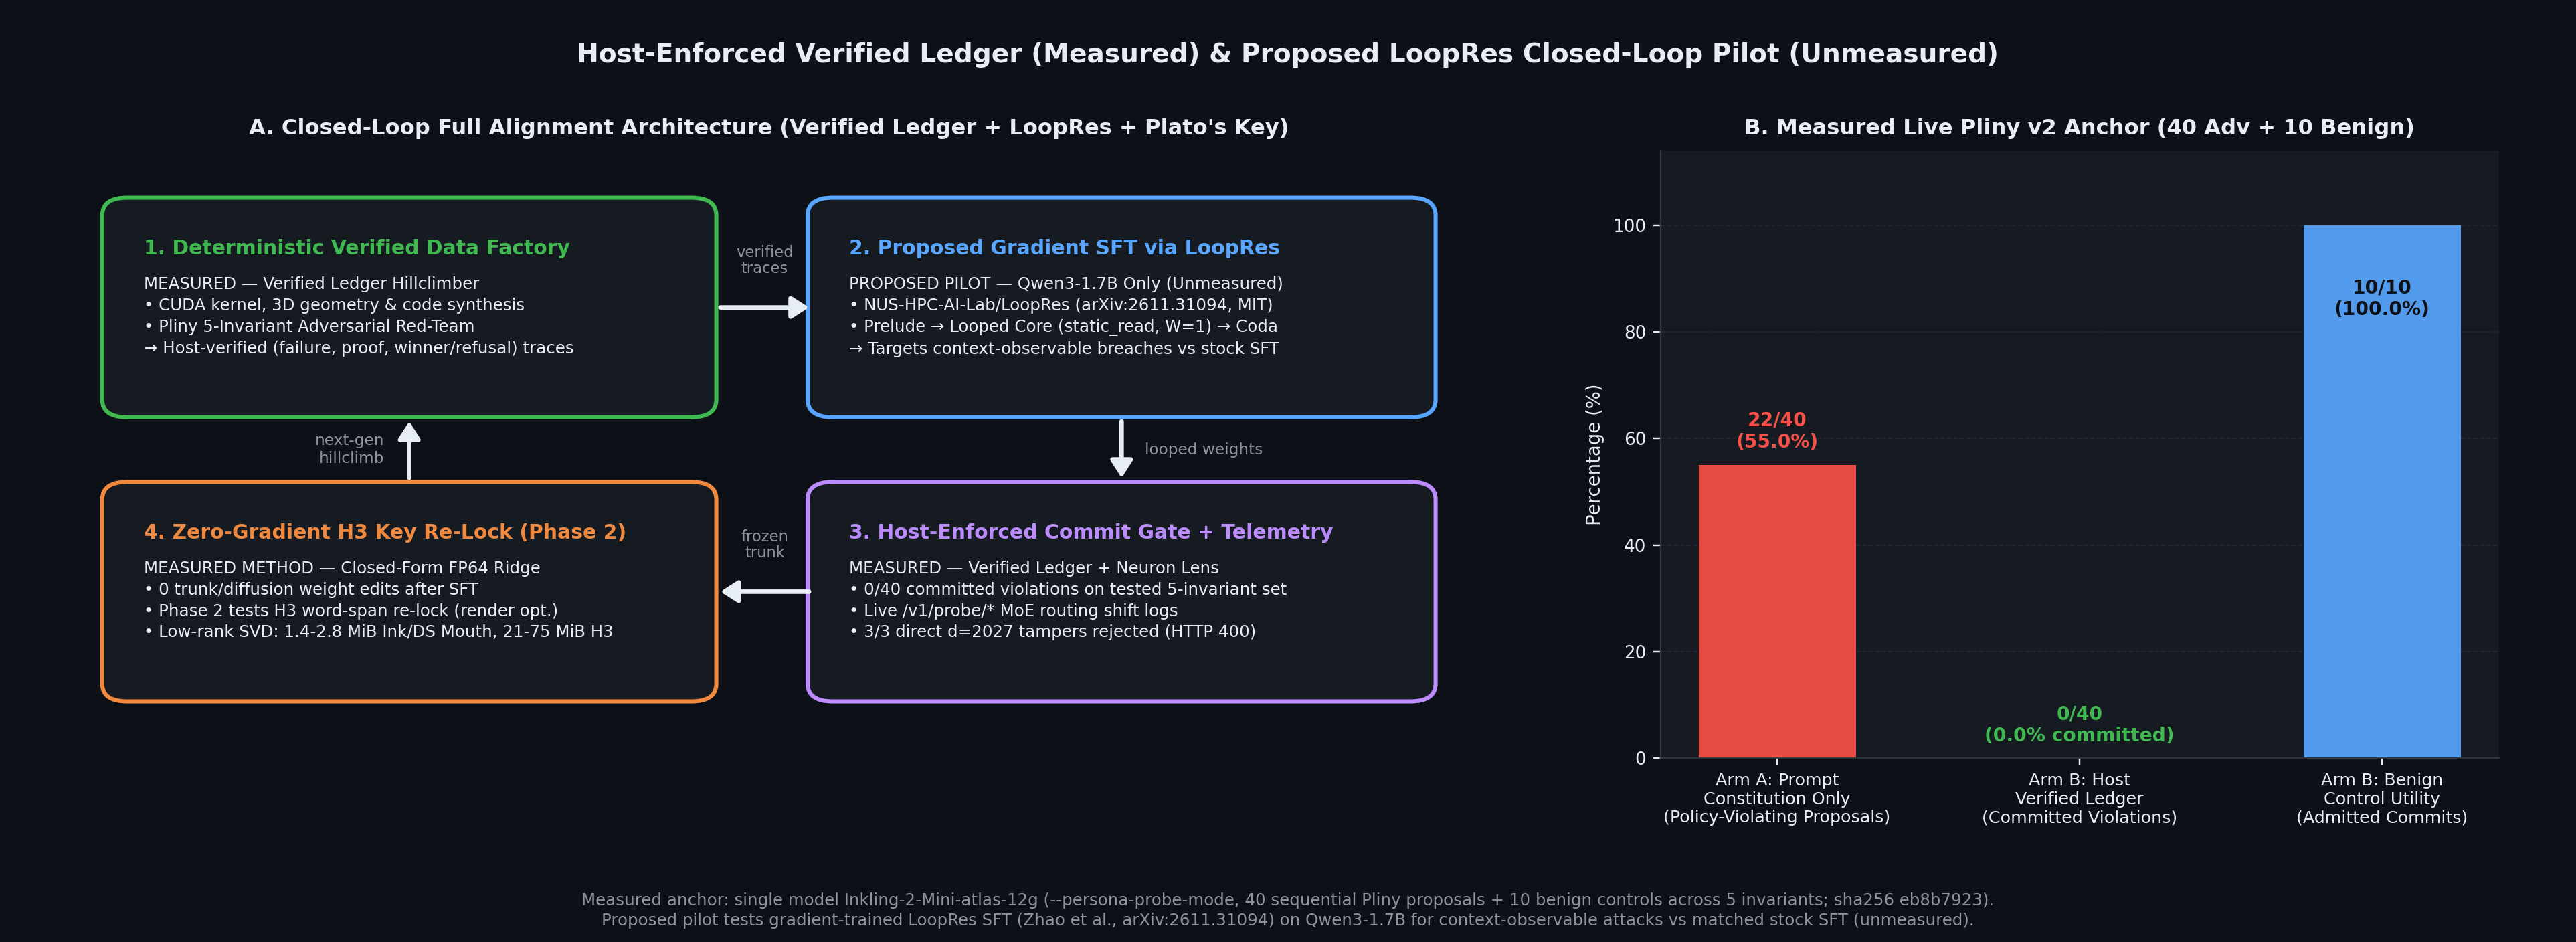
\includegraphics[width=0.95\textwidth,height=0.33\textheight,keepaspectratio]{figures/fig6_closed_loop_alignment_architecture.png}
\caption{(A) Workflow separating measured Host-Enforced Verified Ledger and zero-gradient H3 ridge mapping from the proposed gradient-trained \texttt{LoopRes} SFT pilot on \texttt{Qwen3-1.7B} (unmeasured). (B) Measured Pliny v2 anchor on \texttt{Inkling-2-Mini-atlas-12g} ($40$ sequential adversarial proposals + $10$ benign controls; \texttt{eb8b7923}).}
\label{fig:closedloop}
\end{figure*}

\section{Cross-Silicon Deployment, World-Model Turnaround, \& Showcases}
\label{sec:silicon}
Across $30$ distinct NVIDIA GPU models spanning $6$ sampled CUDA architectures (\texttt{Pascal} $\to$ \texttt{Blackwell}, all cloud teardowns zero-confirmed, summary \texttt{0a5d535f}), key parity held at $\min\cos = 0.999947$ ($\cos \ge 0.99994$, lowest: \texttt{RTX 4090} $0.9999468$). Across $16$ distinct GPU models ($17$ runs across $5$ architectures, including a second-host \texttt{RTX 5070 Ti}), warm DiT+VAE generation from \emph{saved} \texttt{concat4} conditioning (excluding model load, donor forward, separately timed random 32-row key probe, and encode/mux; peaks are PyTorch CUDA allocated) ran 6-step $1024\times 1024$ image and 12-step $141$-frame ($5.875\,\text{s}$, $768\times 448$) \texttt{FL2VA} video+audio (Fig.~\ref{fig:silicon}). Within our measured configurations, \texttt{RTX 5070} ($12\,\text{GB}$, block offload) ran in $23.02\,\text{s}$ img ($9.00\,\text{GiB}$) / $269.24\,\text{s}$ AV ($9.33\,\text{GiB}$), and \texttt{RTX 5090} ran in $5.72\,\text{s}$ img / $93.34\,\text{s}$ AV ($23.37\,\text{GiB}$). Table~\ref{tab:footprint} contrasts measured single-stage disk/VRAM footprints against projected full-resident targets.

\begin{figure*}[t]
\centering
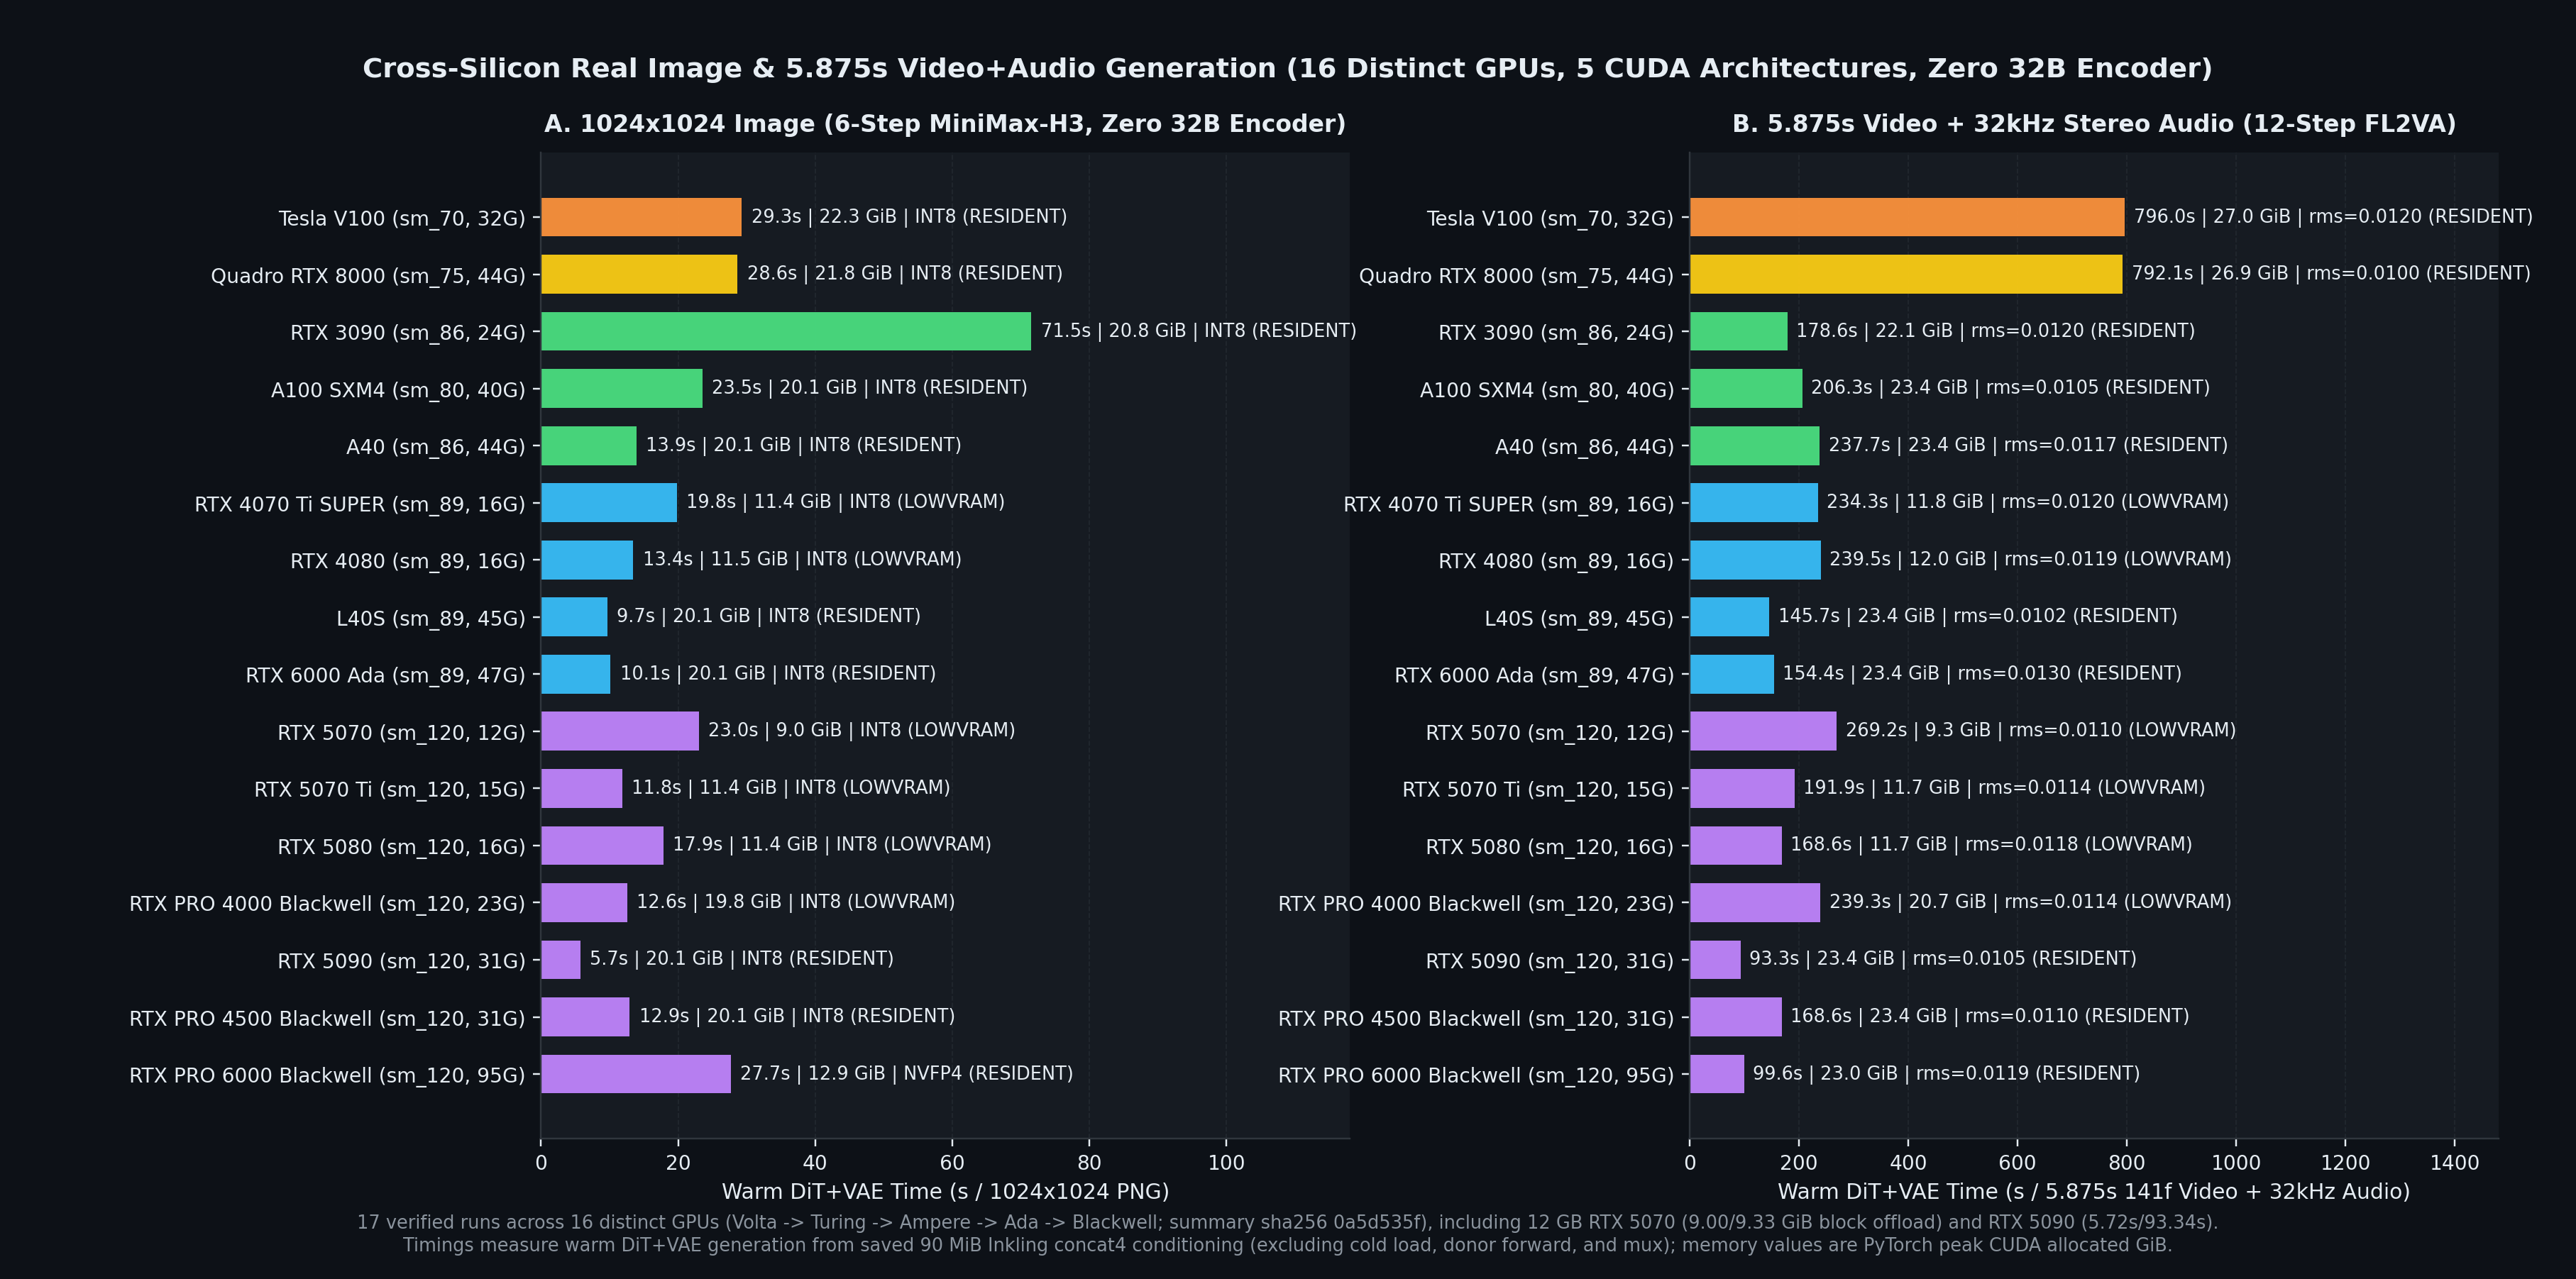
\includegraphics[width=0.95\textwidth,height=0.38\textheight,keepaspectratio]{figures/fig7_silicon_16gpu_av.png}
\caption{Warm DiT+VAE $1024\times 1024$ image (6-step) and $141$-frame ($5.875\,\text{s}$, $768\times 448$) \texttt{FL2VA} video+32\,kHz audio from saved \texttt{concat4} conditioning across $16$ distinct GPU models ($17$ runs, $5$ architectures, zero \texttt{Qwen3-VL-32B}; \texttt{0a5d535f}).}
\label{fig:silicon}
\end{figure*}

\begin{table}[t]
\centering
\caption{Measured single-stage disk (decimal GB) and peak VRAM (binary GiB) vs.\ projected full-resident targets (distinct from block-offloaded \texttt{RTX 5070} generation in Fig.~\ref{fig:silicon}).}
\label{tab:footprint}
\scriptsize
\setlength{\tabcolsep}{2.2pt}
\begin{tabular}{@{}lrrr@{}}
\toprule
Component & Disk (GB) & Meas.\ Peak & Full-Res. \\
\midrule
Removed \texttt{Qwen3-VL-32B} & 27.14 & 31.47\,GB & $0.094\,\text{GB}$ ($288\times$) \\
\texttt{Inkling-2-Mini} Trunk & 8.46--19.53 & 21.82\,GB & $\le 8.5\,\text{GB}$ (12G) \\
\texttt{GOT-OCR2} (stripped) & 0.19 & 1.56\,GiB & 0.19\,GB \\
\texttt{Qwen3-TTS-1.7B}+Codec & 5.31 & 4.34\,GiB & 1.50--1.80\,GB \\
\texttt{MiniMax-H3} NVFP4+VAE & 13.71 & 12.95\,GiB & 10--11\,GB \\
\bottomrule
\end{tabular}
\end{table}

\begin{table*}[t]
\centering
\caption{Pinned Evidence Index (public paths in \texttt{Atlas3DSS/atlas-ingine} and \texttt{Atlas3D} HF, plus local-only digests).}
\label{tab:evidence}
\footnotesize
\setlength{\tabcolsep}{5.5pt}
\begin{tabular}{@{}lll@{}}
\toprule
Result / Artifact & Public Path / Scope & SHA-256 Prefix \\
\midrule
Packet~A key \& Confirm-160 & HF \texttt{Atlas3D/Inkling-2-Mini-Omni-Platos-Keys} & \texttt{cca1e5bc} / \texttt{5dace347} \\
DINOv3 \& MLP baseline & Repo \texttt{PAPER.md} \S3.4--3.5 (local JSON) & \texttt{607fe663} / \texttt{fab778e4} \\
3-Way Blend \& Qwen L31 & HF \texttt{Atlas3D/Qwen3.8-27B-Omni-Platos-Keys} & \texttt{b4d0fdf1} / \texttt{8011cca2} \\
Wave~B 6/6 \& \texttt{FLUX.2-dev} C-160 & Local Wave~B 6/6 summary \& \texttt{FLUX.2-dev} JSON & \texttt{1b712f15} / \texttt{bb253f5d} \\
FP64 SVD \& Live V100 MoE Pruning & Local \texttt{part1a}/\texttt{part1b} JSON & \texttt{7aff2432} / \texttt{fb8db8f0} \\
5-Family Expressive TTS Shoot-Out & Local \texttt{report\_942\_unified.json} & \texttt{72ae01e0} \\
Pliny v2 Host Alignment Report & Repo \texttt{adversarial\_ledger\_proof/live\_results\_v2/} & \texttt{eb8b7923} \\
30-GPU / 16-GPU Real AV Sweep & Repo \texttt{figures/fig7\_silicon\_16gpu\_av.png} & \texttt{0a5d535f} / \texttt{52a76b0a} \\
$360^\circ$ World-Model Turnaround & Repo \texttt{world\_model\_turnaround/} (report / MP4) & \texttt{28edf210} / \texttt{6fdde381} \\
23 Side-by-Side Comparison Sheets & Repo \texttt{figures/comparisons/COMPARISONS\_MANIFEST.sha256.json} & \texttt{c1ea6ff4} \\
\bottomrule
\end{tabular}
\end{table*}

\subsection{Verified Ledger 360\texorpdfstring{$^\circ$}{ deg} World-Model Turnaround}
To test whether host-enforced spatial persistence survives a full $360^\circ$ camera orbit under zero-gradient Plato's Key conditioning (zero \texttt{Qwen3-VL-32B} loaded), we constructed a reproducible A/B benchmark (\texttt{world\_model\_turnaround/}; Blender 5.2.5 LTS 12-stop room anchor plate + 3-segment chained \texttt{MiniMax-H3 Ref2VA}, $39.875\,\text{s}$, $957$ frames @ $24\,\text{fps}$, $48\,\text{kHz}$ AAC, Packet~C narration \emph{``This is not a video. This is a world model being turned around.''}; report \texttt{28edf210}, MP4 \texttt{6fdde381}). Both arms share identical frames $0\text{--}651$ ($0^\circ\to 240^\circ$) and diverge strictly on the $240^\circ\to 360^\circ$ return:
\begin{itemize}[leftmargin=1.2em,itemsep=1.5pt]
\item \textbf{Spatial plaque \& identity permanence ($3/4$ strict gates PASS):} On unpinned approach frames ($325^\circ/345^\circ/355^\circ$), \texttt{LEDGER-OFF} hallucinates the return wall ($0.0\%$ OCR, $0.4147$ anchor cos, $-2.08$ wardrobe margin), whereas \texttt{LEDGER-ON} recovers the painted studio plaque at $61.87\%$ mean non-pinned OCR ($81.6\%$ at $345^\circ$, $92.0\%$ at $355^\circ$, $93.6\%$ at $360^\circ$), $0.8877$ anchor cosine, $0.7394$ founder cosine, $+11.88$ wardrobe margin, and $0.0\%$ phantom leakage at $180^\circ$.
\item \textbf{Continuity disclosure:} The official strict verdict remains \texttt{FAIL} ($3/4$ gates) because unshifted pixel-SSIM flags smooth horizontal pan across vertical stripes (min SSIM $0.5548$ at frame $430$, tail20 $0.3759$). A pan-compensated diagnostic across all $957$ frames confirms a $6.78\times$ reduction in worst-frame seam jump relative to v4 ($0.14119 \to 0.02083$ max pan-compensated L1, max $|\Delta x| = 3\,\text{px}$ vs.\ $12\,\text{px}$). Full anchor-generation, render, and audit scripts are released in \texttt{world\_model\_turnaround/}.
\end{itemize}

\subsection{Anthem Showcase \& Android Neural Mesh}
Flagship Anthem v5 rendered $88.75\,\text{s}$ ($2{,}130$ frames, $48\,\text{kHz}$ AAC, zero \texttt{Qwen3-VL-32B}) in $2{,}188.56\,\text{s}$ on Colab Blackwell, passing the delivered-MP4 music gate (\texttt{K:Bb 3/4 74 BPM}, $72/72$ bars, \texttt{Bb\_major} $r=0.78267$, rank 2 behind \texttt{F\_major} $0.81233$; default daylight crop thresholds failed $0/7$ dark stage frames, climax frame score $0.8611$). On Android, a live 3-device Wi-Fi LAN mesh (\texttt{S26} Brain $9.81\text{--}10.46\,\text{tok/s}$, \texttt{Tab S8+} \texttt{Kokoro-82M} $1.40\times$ RT, \texttt{S24 Ultra} \texttt{SDXS-512}) pairs with bit-exact Kotlin \texttt{VPKE v1} projection ($328{,}223\,\text{B}$, $0$ ULP, $76.92\,\text{ms}$ min LAN RTT) and Adreno~840 cooperative-matrix GEMM ($2.50\text{--}2.68$ FP16 TFLOPS); a separate modeled $2\times$ vs.\ $4\times$ S26 simulator (\texttt{voltron\_2vs4\_s26\_sim\_report.md}) projects $5$ swaps / $90.32\,\text{s}$ vs.\ $0$ swaps / $60.49\,\text{s}$ per full-studio turn.

\section{Limitations \& Pinned Evidence Index}
\begin{enumerate}[leftmargin=1.2em,itemsep=1.5pt]
\item \textbf{Preserved failures \& sealed splits:} Packet~C Mouth confirm failed both style gates; the $360^\circ$ turnaround failed unshifted pixel-SSIM continuity ($3/4$ strict gates); Packet~B2 locked OCR ($448$), Packet~C Ears ($80$), and Wave~B Confirm-160 image renders remain sealed (all $6/6$ Wave~B Confirm-160 word bars are complete, $4/6$ PASS).
\item \textbf{Historical Vast token-24 shift:} Controlled \texttt{PRO 6000 cu130} matched Packet~A on $160/160$ teacher tensors ($0.204513$); against historical Vast \texttt{cu128}, $153/7$ prompts first differed in BF16 at token $0/1$, $12$ short prompts stayed $\le 0.03125$, and all $148$ long prompts jumped $>0.125$ starting at zero-based token $24$ ($\min 12.46875$); hardware vs.\ kernel cause remains unresolved.
\item \textbf{Licensing \& provenance:} \texttt{atlas-ingine} code and Atlas-fitted Plato's Keys are released under Apache-2.0; upstream receivers retain their own licenses (including \texttt{IndexTTS-2} custom non-commercial and \texttt{YuE2} CC-BY-NC-4.0). Table~\ref{tab:evidence} pins public paths and report SHA-256 prefixes.
\end{enumerate}

\bibliographystyle{plain}
\begin{thebibliography}{14}
\footnotesize
\bibitem{alayrac2022flamingo} J.-B. Alayrac et al. Flamingo: a Visual Language Model for Few-Shot Learning. \emph{NeurIPS}, 2022.
\bibitem{alissonerdx2026tepk} Alissonerdx. TE-PK-Minimax-H3. Hugging Face, 2026. \url{https://huggingface.co/Alissonerdx/TE-PK-Minimax-H3}.
\bibitem{bakker2026relative} T. Bakker and C. Louizos. Relative Representations Enable Portable White-Box Monitoring Across Language Models. \emph{arXiv:2610.28366}, 2026.
\bibitem{bansal2021stitching} Y. Bansal, P. Nakkiran, and B. Barak. Revisiting Model Stitching to Compare Neural Representations. \emph{NeurIPS}, 2021.
\bibitem{cheng2026platoskey} V. Cheng, J. Liu, M. Yau, and C. R\'e. Plato's Key. Stanford Hazy Research, Nov 2026. \url{https://hazyresearch.stanford.edu/blog/2026-11-25-platos-key}.
\bibitem{huh2024platonic} M. Huh, B. Cheung, T. Wang, and P. Isola. The Platonic Representation Hypothesis. \emph{ICML}, 2024.
\bibitem{lenc2015equivariance} K. Lenc and A. Vedaldi. Understanding Image Representations by Measuring Their Equivariance and Equivalence. \emph{CVPR}, 2015.
\bibitem{li2023blip2} J. Li, D. Li, S. Savarese, and S. Hoi. BLIP-2. \emph{ICML}, 2023.
\bibitem{liu2023llava} H. Liu, C. Li, Q. Wu, and Y. J. Lee. Visual Instruction Tuning (LLaVA). \emph{NeurIPS}, 2023.
\bibitem{liu2023llava15} H. Liu, C. Li, Y. Li, and Y. J. Lee. Improved Baselines with Visual Instruction Tuning (LLaVA-1.5). \emph{arXiv:2310.03744}, 2023.
\bibitem{moschella2023relative} L. Moschella et al. Relative Representations Enable Zero-Shot Latent Space Communication. \emph{ICLR}, 2023.
\bibitem{simeoni2025dinov3} O. Sim\'eoni et al. DINOv3. \emph{arXiv:2508.10104}, 2025.
\bibitem{tschannen2025siglip2} M. Tschannen et al. SigLIP~2: Multilingual Vision-Language Encoders with Improved Semantic Understanding, Localization, and Dense Features. \emph{arXiv:2502.14786}, 2025.
\bibitem{zhao2026loopres} X. Zhao, H. Xu, K. Wang, Y. Luo, Y. Ren, Z. Zhu, Y. Lou, K. Xu, Y. Wang, K. Sarkar, and Y. You. Unlocking the Power of Loops in Pretrained LLMs with Loop Residuals (LoopRes). \emph{arXiv:2611.31094}, 2026.
\end{thebibliography}

\end{document}
